
\PassOptionsToPackage{table}{xcolor}
\documentclass{article}

\usepackage[francais]{babel}
\usepackage[T1]{fontenc}
\usepackage[utf8]{inputenc}
\usepackage{xcolor}
\usepackage{graphicx}
\usepackage[colorlinks=true]{hyperref}
\hypersetup{urlcolor=blue,linkcolor=red,colorlinks=false} 
\usepackage{algorithm,algorithmic}
\usepackage{listings}
\usepackage{amssymb}
\usepackage{setspace}
\usepackage{listings}
\usepackage{lscape}
\usepackage{amsmath}
\usepackage{wrapfig}
\usepackage[margin=2.5cm]{geometry}


% Romain
\newcommand{\cRM}[1]{\MakeUppercase{\romannumeral #1}}  % Capital
\newcommand{\cRm}[1]{\textsc{\romannumeral #1}} % Petit majuscule
\newcommand{\crm}[1]{\romannumeral #1}
% Siècle %
\newcommand{\siecle}[1]{\cRM{#1}\textsuperscript{e}~siècle}


\definecolor{keywords}{RGB}{255,0,0}
\lstset{language=[LaTeX]TeX,
texcsstyle=*\color{keywords},
breaklines=true,
keywordstyle=\color{keywords},
commentstyle=\color{darkgreen},
tabsize=2,
backgroundcolor=\color{lightgrey},
escapeinside=||,
morekeywords={*,subsection,make title,tableofcontents,include graphics}
}


\rowcolors{1}{gray!25}{white}

\title{Les stratégies militaires dans les Systèmes Multi-Agents}
\author{Chloé Desdouits, William Dyce}
\date{\today}


\begin{document}


\maketitle

\tableofcontents
\newpage


\section{Organisations guerrières}
Il y a deux types d'organisations militaires bien différents : les armées et les guérillas. Nous allons présenter pour chaque type sa structure et le contexte dans lequel il existe.

\subsection{Armées}
Les armées sont des entités qui tirent leur légitimité de leur appartenance aux états ou jadis aux institutions religieuses.

\subsubsection{Structure}
La structure des armées est homogène : en effet, la hiérarchie est sous forme d'arbre dont les nœuds du même niveau ont le même nombre de fils.
\begin{figure}[H]
	\begin{centering}
	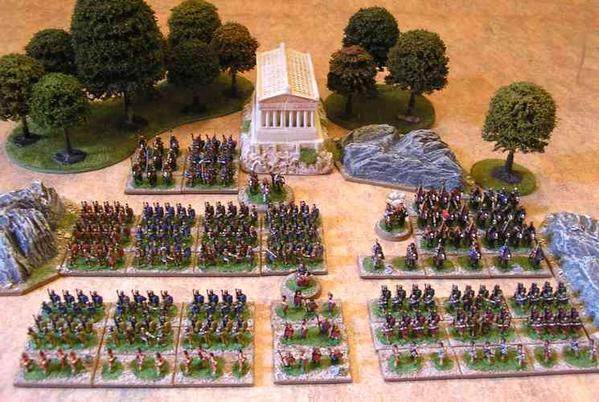
\includegraphics[width=0.8\linewidth]{../ressources/armee_cesar}
	\caption{Exemple d'organisation homogène de l'armée (armée de César - Warmaster ancients \cite{armee_de_cesar})}
	\end{centering}
\end{figure}

Cela permet de construire des formations à grande échelle qui aient une structure prédéfinie.
\begin{figure}[H]
\begin{centering}
\begin{tabular}{| c l | c l | c l | c l |}
	\hline
	\multicolumn{8}{| c |}{\textbf{Armée}}
	\\
	\multicolumn{2}{| c |}{\textbf{Spartiate}} 	& \multicolumn{2}{ c |}{\textbf{Romaine}} & \multicolumn{2}{ c |}{\textbf{Perse}}	& \multicolumn{2}{ c |}{\textbf{Mongole}} 	\\
	\hline
	 					&			& 					&			& 				&			& \textit{Ordu}		& > 10000			\\
	 \itshape Mora 			& 576		& \itshape Légion		& 6000		& \textit{Baivarabam}& 10000		& \textit{Tumen} 	& 10000			\\
	 \itshape Loche			& 144		& \itshape Cohorte		& 600		& \textit{Hazarabam}	& 1000		& \textit{Minghan}  	& 1000			\\
	 \itshape Pentécostye	& 72			& \itshape Manipule		& 200		& \textit{satabam}	& 100		& \textit{Zuut} 		& 100			\\
	 \itshape Énomotie		& 36			& \itshape Centurie		& 100		& \textit{Dathabam} 	& 10			& \textit{Arav} 		& 10				\\
	\hline
\end{tabular}
\caption{Effectif des unités dans différentes armées antiques \cite{mongol_army, spart_army, roman_legion,persian_army}}
\end{centering}
\end{figure}


\subsubsection{Contexte}
Les armées interviennent dans deux contextes principaux : la défense de la patrie et la conquête de nouveaux territoires.
\begin{figure}[H]
	\begin{centering}
	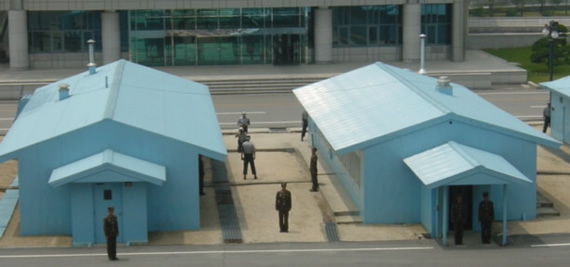
\includegraphics[width=\linewidth]{../ressources/dmz-corea}
	\caption{Zone démilitarisée entre la Corée du Sud et la Corée du Nord \cite{dmz_corea}}
	\end{centering}
\end{figure}
\begin{figure}[H]
	\begin{centering}
	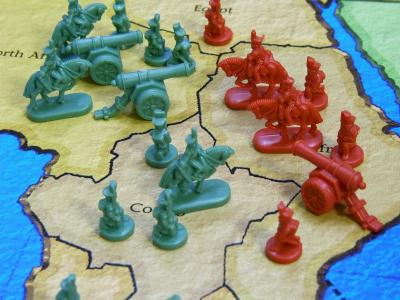
\includegraphics[]{../ressources/risk-board-game}
	\caption{Tentative de conquête dans le jeu Risk \cite{risk_picture}}
	\end{centering}
\end{figure}




\subsection{Guérillas}
Les guérillas se forment à la suite d'une scission idéologique entre le pouvoir en place et une partie de la population. Elles ont souvent à leur tête un leader charismatique.

\subsubsection{Structure}
Ces organisation sont souvent structurées de façon très hétérogène : peu de responsables et des formations à petite échelle.
\begin{figure}[H]
	\begin{centering}
	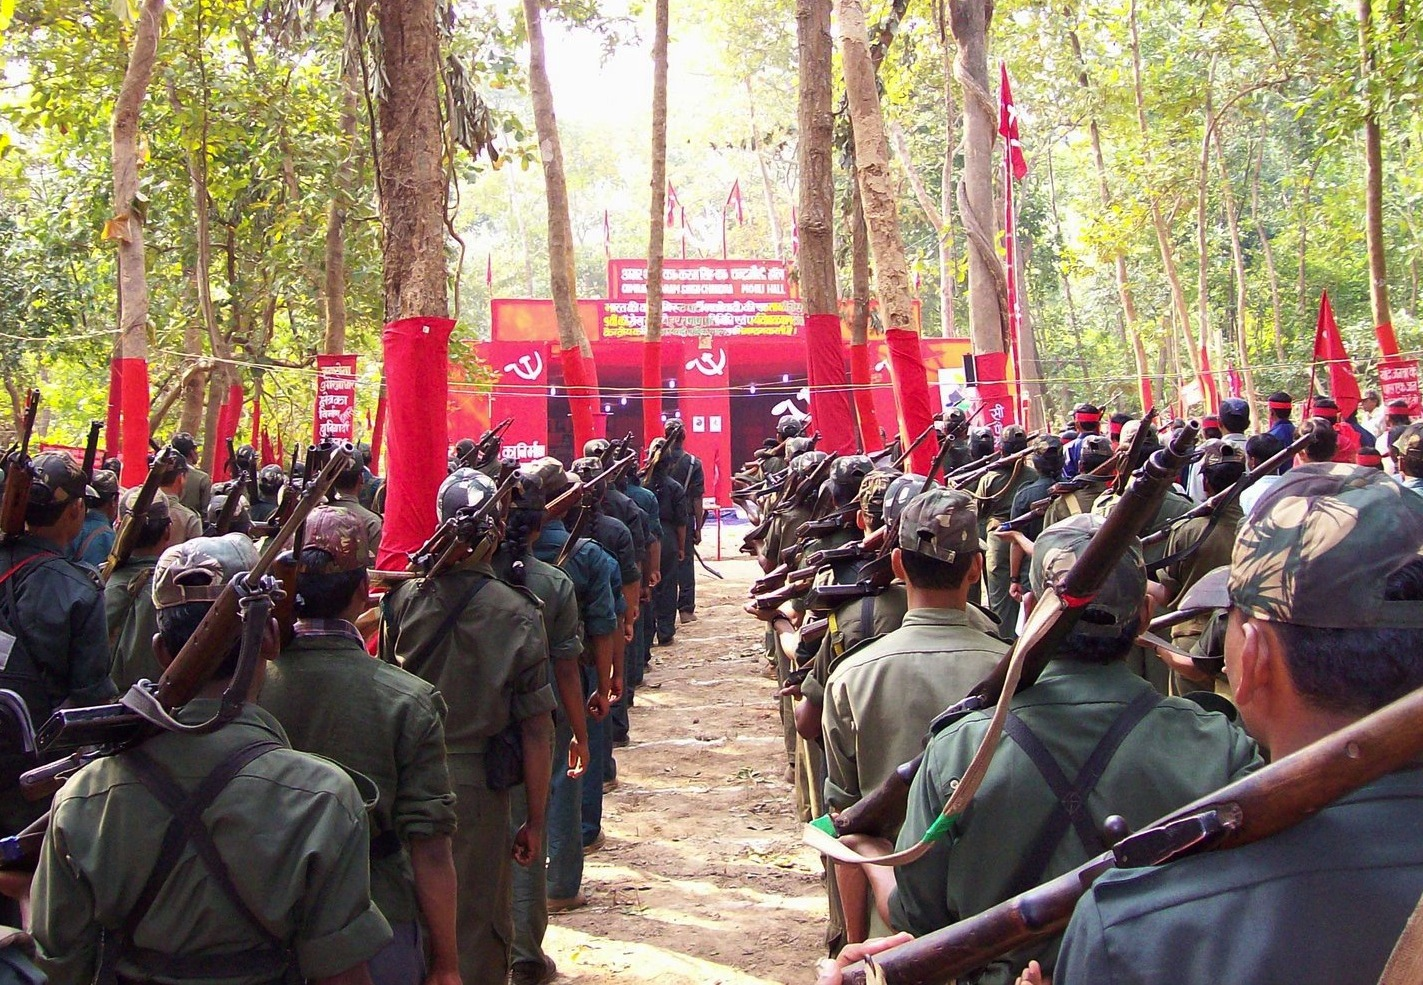
\includegraphics[width=\linewidth]{../ressources/guerrilla_naxalite}
	\caption{Guérilla Naxalite (Inde) \cite{guerrilla_naxalite}}
	\end{centering}
\end{figure}

Les guérillas, comme le montre la figure suivante, ont une échelle réduite par rapport aux forces contre lesquelles elles luttent.
\begin{figure}[H]
	\begin{centering}
	\begin{tabular}{| l | c | c | c | c |}
	\hline
	\textbf{Localisation}		& \textbf{Irlande} 	& \textbf{Inde} 	& \textbf{Cuba}	& \textbf{Colombie}	\\
	\hline
	\textbf{Régime}			& 55.000			& 1.414.000	& 35.000		& 300.000			\\
	\textbf{Insurgés}		& 15.000			& 15.000		& 200		& 20.000			\\
	\hline
	\end{tabular}
	\caption{Effectifs des forces du régime par rapport aux forces des guérillas \cite{naxalite_guerrilla_wiki, irish_civil_war_wiki}}
	\end{centering}
\end{figure}


\subsubsection{Contexte}
Les forces de guérilla sont adaptées au terrain : montagnes, maquis, villes \ldots
\begin{figure}[H]
	\begin{centering}
	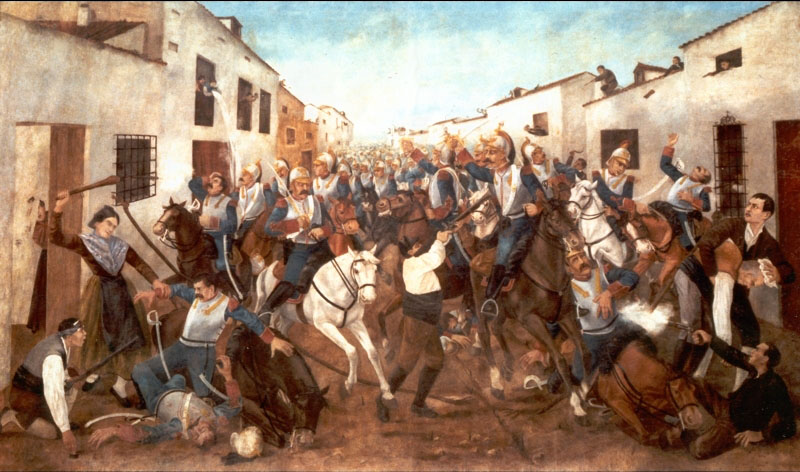
\includegraphics[width=\linewidth]{../ressources/valdepenas}
	\caption{Soulèvement de Valdepeñas ; guérilla urbaine \cite{valdepenas}}
	\end{centering}
\end{figure}
Elles sont mobiles.
\begin{figure}[H]
	\begin{centering}
	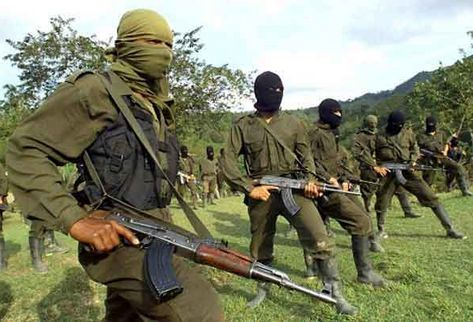
\includegraphics[]{../ressources/guerrilla_colombia}
	\caption{Guérilla colombienne \cite{guerrilla_colombia}}
	\end{centering}
\end{figure}
La plupart des recrues sont des civils.
\begin{figure}[H]
	\begin{centering}
	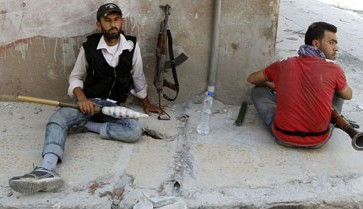
\includegraphics[]{../ressources/rebel_syrie}
	\caption{Des rebelles en Syrie \cite{rebel_syrie}}
	\end{centering}
\end{figure}


\section{Stratégies militaires}

\subsection{Définitions}
Politique \cite{politique_jomini}
\begin{quote}“La politique de la guerre c’est tout simplement décider où, quand, comment, avec quels alliés et pourquoi entrer en guerre.”\end{quote}
\begin{figure}[H]
	\begin{centering}
	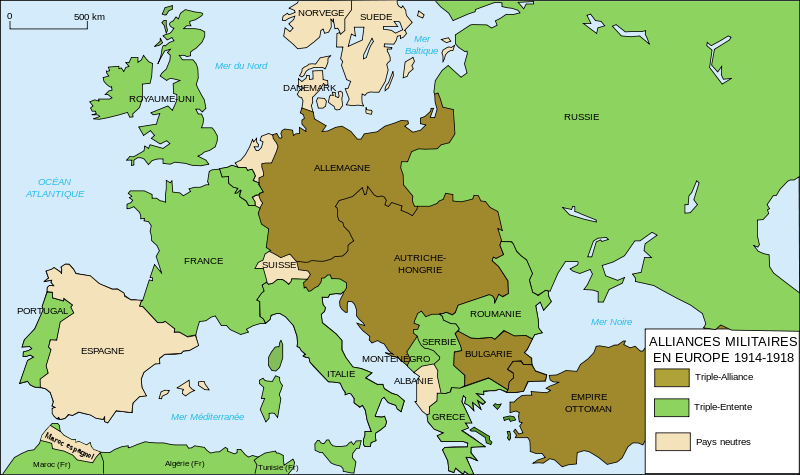
\includegraphics[width=\linewidth]{../ressources/alliances_ww1}
	\caption{Alliances militaires en Europe 1914-1918 \cite{ww1}}
	\end{centering}
\end{figure}

Stratégie \cite{military_strategy}
\begin{quote}“La stratégie militaire est l'art de coordonner -au plus haut niveau de décision- l'action de l'ensemble des forces militaires de la Nation pour conduire une guerre, gérer une crise ou préserver la paix.”\end{quote}
\begin{figure}[H]
	\begin{centering}
	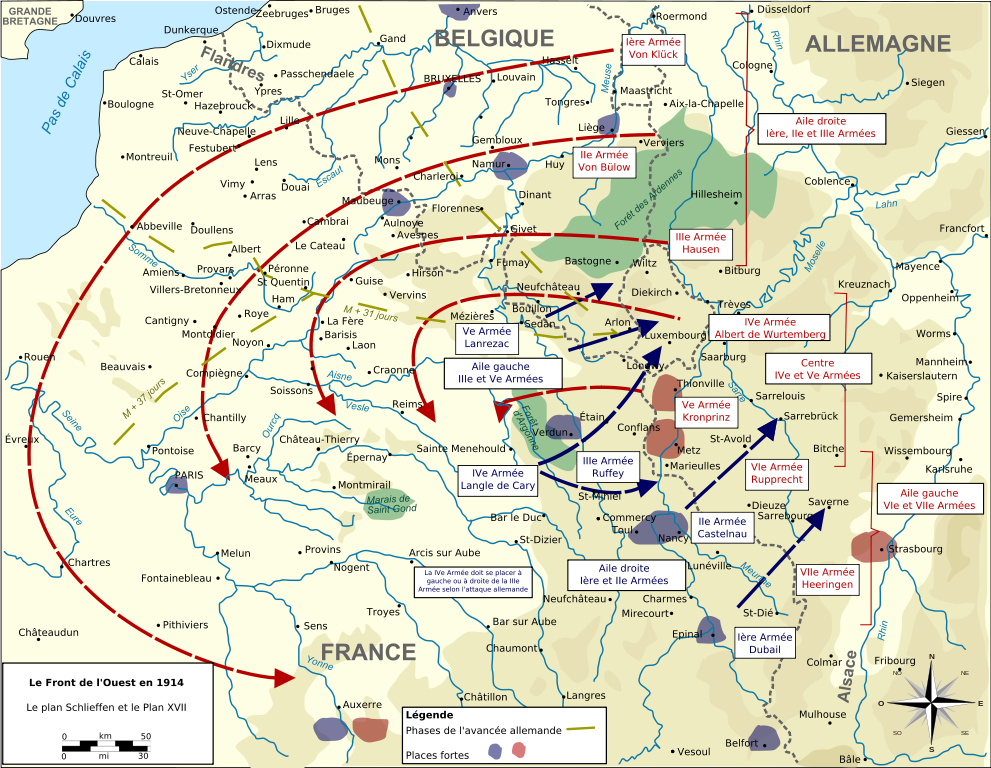
\includegraphics[width=\linewidth]{../ressources/strategy_ww1}
	\caption{Plans de bataille des états-majors allemand et français pendant la WW1 \cite{ww1}}
	\end{centering}
\end{figure}

Tactique \cite{tactic}
\begin{quote}“La tactique est l'art de diriger une bataille, en combinant, par la manœuvre, l'action des différents moyens de combat en vue d'obtenir le maximum d'efficacité.”\end{quote}
\begin{figure}[H]
	\begin{centering}
	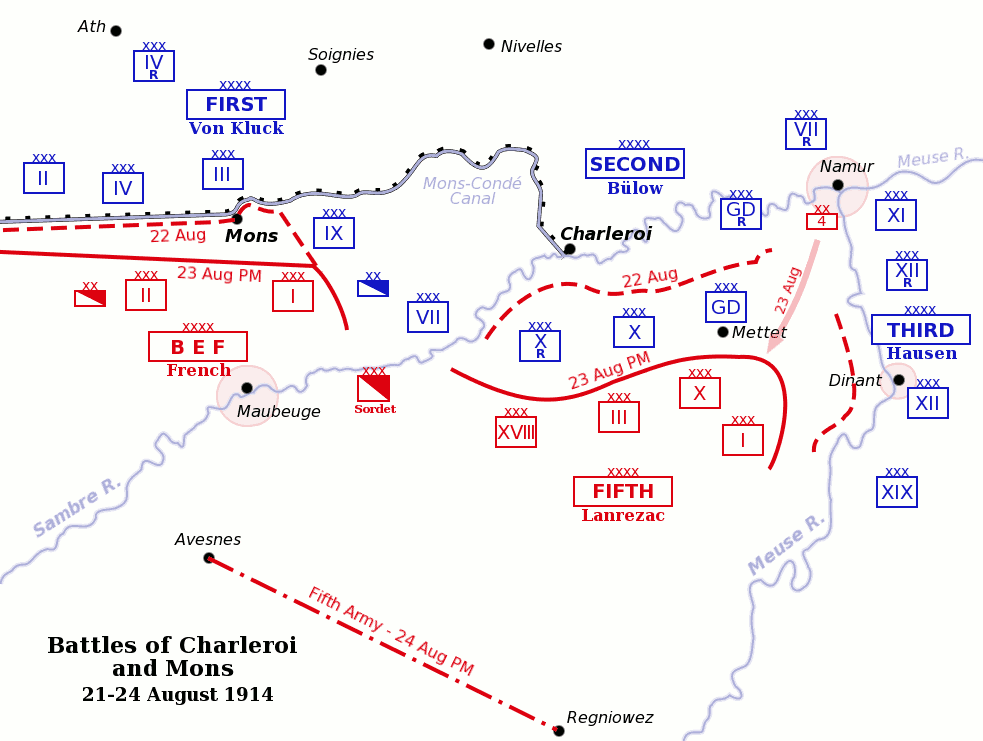
\includegraphics[width=\linewidth]{../ressources/Battles_of_Charleroi_ww1}
	\caption{Mouvement de troupes pendant la bataille de Charleroi (WW1) \cite{charleroi_battle}}
	\end{centering}
\end{figure}



\subsection{Stratégies}

\subsubsection{Sun Tzu}
Chine (\siecle{6} BC) \hfill \begin{minipage}{5cm}
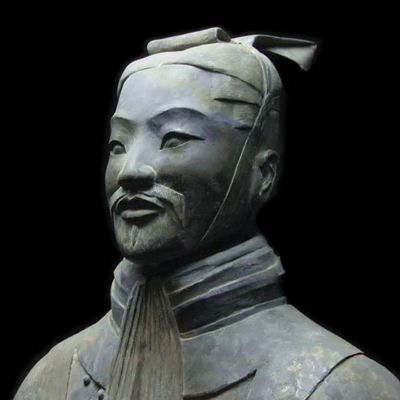
\includegraphics[width=\linewidth]{../ressources/sun_tzu_general}
\end{minipage}
\begin{quote}“L'art de la guerre, c'est de soumettre l'ennemi sans combat.”\end{quote}

Préceptes
\begin{itemize}
\item prendre toutes les possessions de l'adversaire et les conserver intactes
\item adaptabilité, préparation, connaissance du terrain et des forces en présence (espionnage)
\end{itemize}
Axes stratégiques
\begin{enumerate}
\item cause morale
\item conditions climatiques
\item conditions géographiques
\item qualités du dirigeant
\item organisation et discipline
\end{enumerate}

\cite{tzu1997art, sun_tzu_fighting, sun_tzu_wiki}

\subsubsection{Alexandre le grand}
Grèce (\siecle{4} BC)
\hfill \begin{minipage}{5cm}
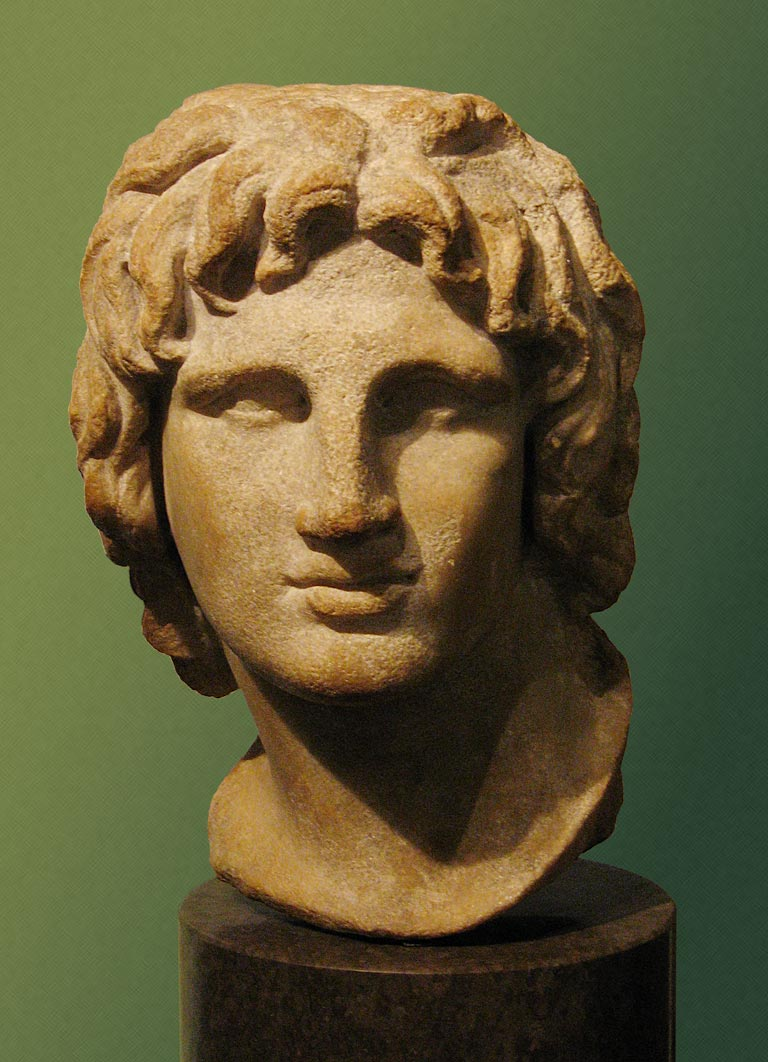
\includegraphics[width=\linewidth]{../ressources/AlexanderTheGreat_Bust}
\end{minipage}
\begin{quote}“Ce qui ne me tue pas me rend plus fort.”\end{quote}

Préceptes
\begin{itemize}
\item conscription et intégration des peuples vaincus
\item allègement de l'équipement des troupes
\end{itemize}
Axes stratégiques
\begin{enumerate}
\item assurer ses arrières
\item choisir judicieusement la voie d'accès pour chaque conquête
\end{enumerate}
\cite{alexander_the_great, alexandre_balkans}

\subsubsection{Julius Caesar}
Italie (\siecle{1} BC)
\hfill \begin{minipage}{5cm}
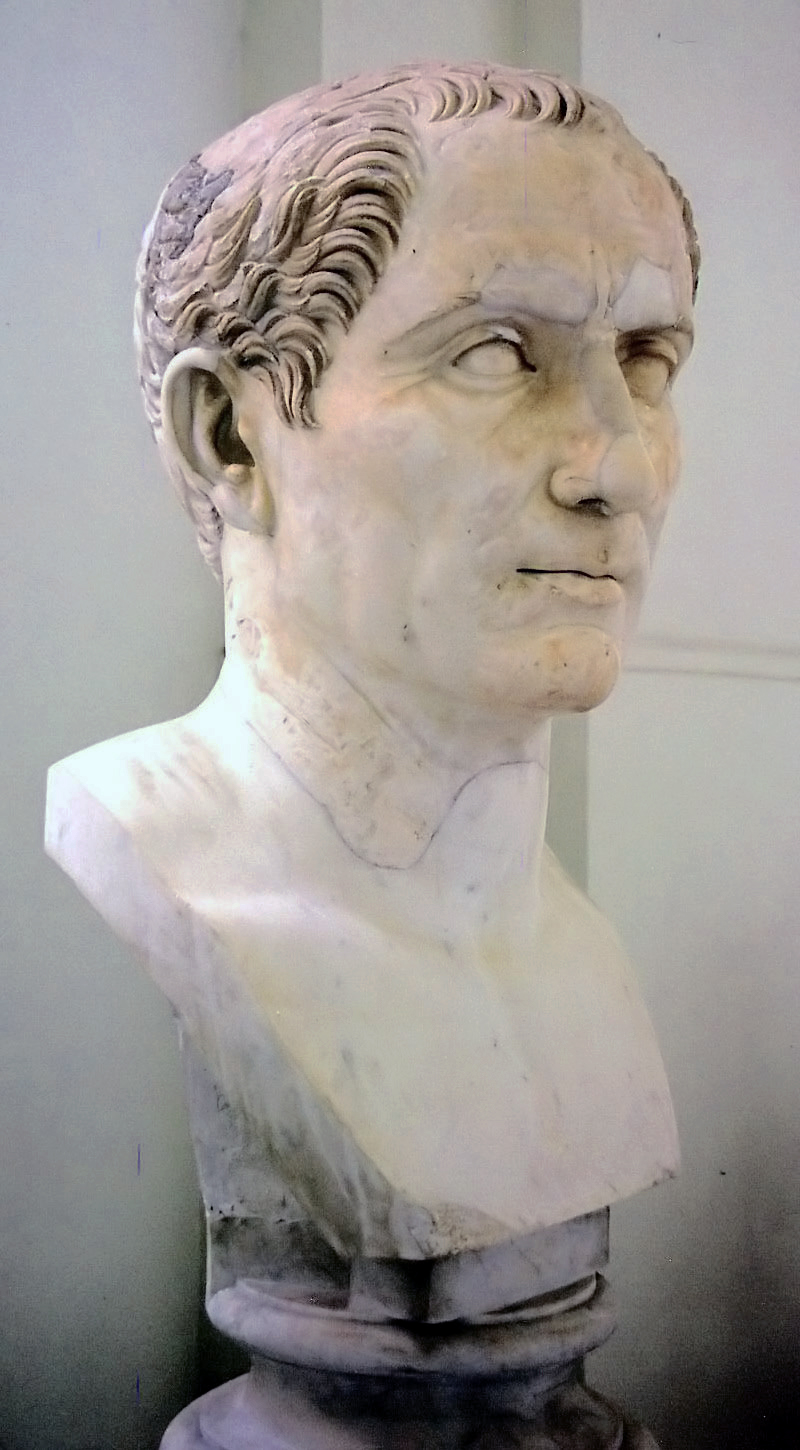
\includegraphics[width=\linewidth]{../ressources/cesare}
\end{minipage}
\begin{quote}“L’expérience, voilà le maître en toutes choses.”\end{quote}

Préceptes
\begin{itemize}
\item stabilité militaire et logistique
\end{itemize}
Axes stratégiques
\begin{enumerate}
\item infanterie lourde
\item bataillons étrangers spécialisés
\item formations en fonction des conditions géographiques
\item bivouac fortifié
\end{enumerate}
\cite{caesar_wiki, caesar_lacks}

\subsubsection{Genghis Khan}
Mongolie (\siecle{12})
\hfill \begin{minipage}{5cm}
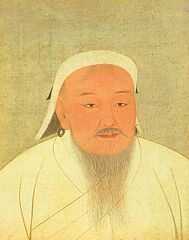
\includegraphics[width=\linewidth]{../ressources/genghis_khan}
\end{minipage}
\begin{quote}“Le plus grand bonheur du Mongol est de vaincre l’ennemi, de ravir ses trésors, de faire hurler ses serviteurs, de se sauver au galop de ses chevaux bien nourris [\ldots]”\end{quote}

Préceptes
\begin{itemize}
\item guerre psychologique
\item règne de la terreur
\item connaissance du terrain : espionnage ; éclaireurs
\end{itemize}
Axes stratégiques
\begin{enumerate}
\item peu de troupes ; avant-garde forte
\item troupes montées % logistique et vitesse
\item délégation des décisions
\item relais de communication et ravitaillement
\item attaques biologiques
\end{enumerate}
\cite{khan_wiki, military_strategy, mongol_army}

\subsubsection{Napoléon Bonaparte}
France (\siecle{18})
\hfill \begin{minipage}{5cm}
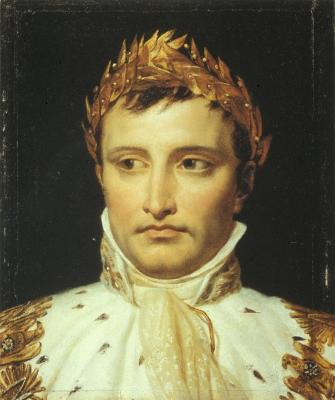
\includegraphics[width=\linewidth]{../ressources/napoleon}
\end{minipage}
\begin{quote}“Réunir ses feux contre un seul point ; une fois la brèche faite, l’équilibre est rompu, tout le reste devient inutile.”\end{quote}
Préceptes
\begin{itemize}
\item recherche systématique de la bataille
\item destruction totale des forces adverses
\item être le plus fort à l’endroit où l’on a décidé de frapper le coup décisif
\end{itemize}
Axes stratégiques
\begin{enumerate}
\item vitesse de manœuvre : {\emph Blitzkrieg}
\item fortifications
\item lignes de réapprovisionnement provisoires
\item artillerie
\end{enumerate}
\cite{napoleon, napoleon_wiki, napoleon_portrait}


\subsubsection{Conclusion}

\begin{tabular}{|p{0.45\linewidth}|p{0.45\linewidth}|}
\hline
\emph{Stratégie indirecte} & \emph{Stratégie directe}\\
\hline
renseignement & conscription\\
embuscade & recherche de la bataille décisive\\
tromperie & planification et formations\\
sabotage & fortifications\\
\hline
\end{tabular}

\begin{figure}[H]
	\begin{centering}
	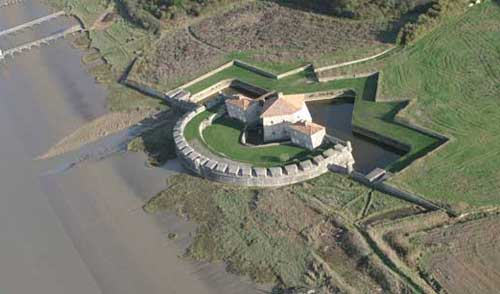
\includegraphics[width=0.8\linewidth]{../ressources/Vauban_Fort_Lupin}
	\caption{Vue aérienne du Fort Lupin construit par Vauban (Rochefort). \cite{fort_lupin}}
	\end{centering}
\end{figure}
\begin{figure}[H]
	\begin{centering}
	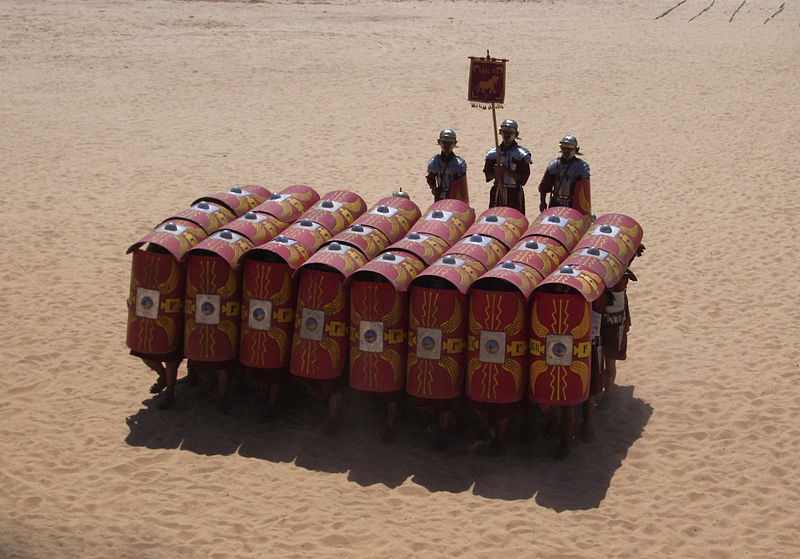
\includegraphics[width=\linewidth]{../ressources/tortue}
	\caption{La tortue : formation défensive romaine. \cite{turtle_form}}
	\end{centering}
\end{figure}
\begin{figure}[H]
	\begin{centering}
	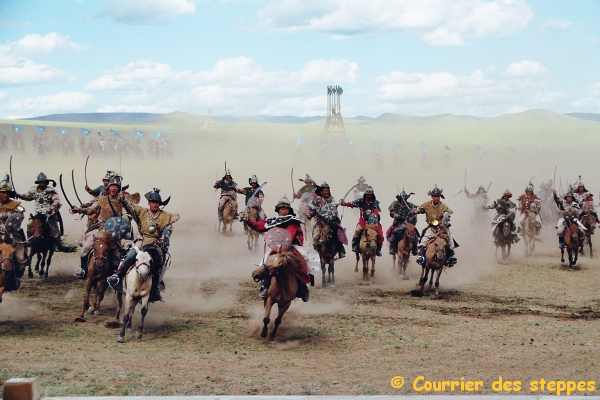
\includegraphics[width=\linewidth]{../ressources/mongol_army}
	\caption{Charge de cavalerie mongole. \cite{mongol_cavalery}}
	\end{centering}
\end{figure}
\begin{figure}[H]
	\begin{centering}
	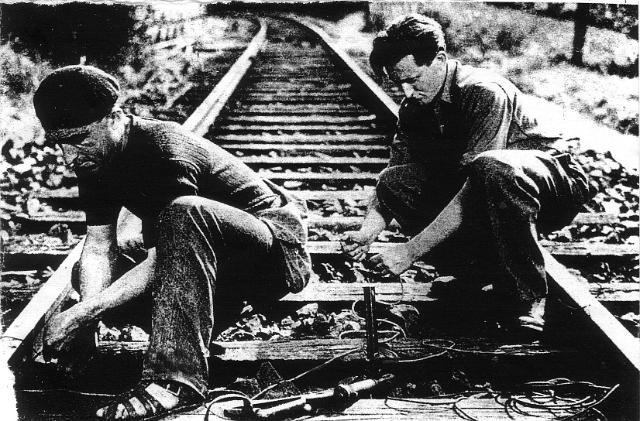
\includegraphics[width=\linewidth]{../ressources/sabotage_maquisards}
	\caption{Sabotage d'une voie de chemin de fer - guerre de 1914. \cite{sabotage}}
	\end{centering}
\end{figure}
\cite{war}


\subsection{Formations et unités}

\subsubsection{Infanterie}
\begin{figure}[H]
	\begin{centering}
	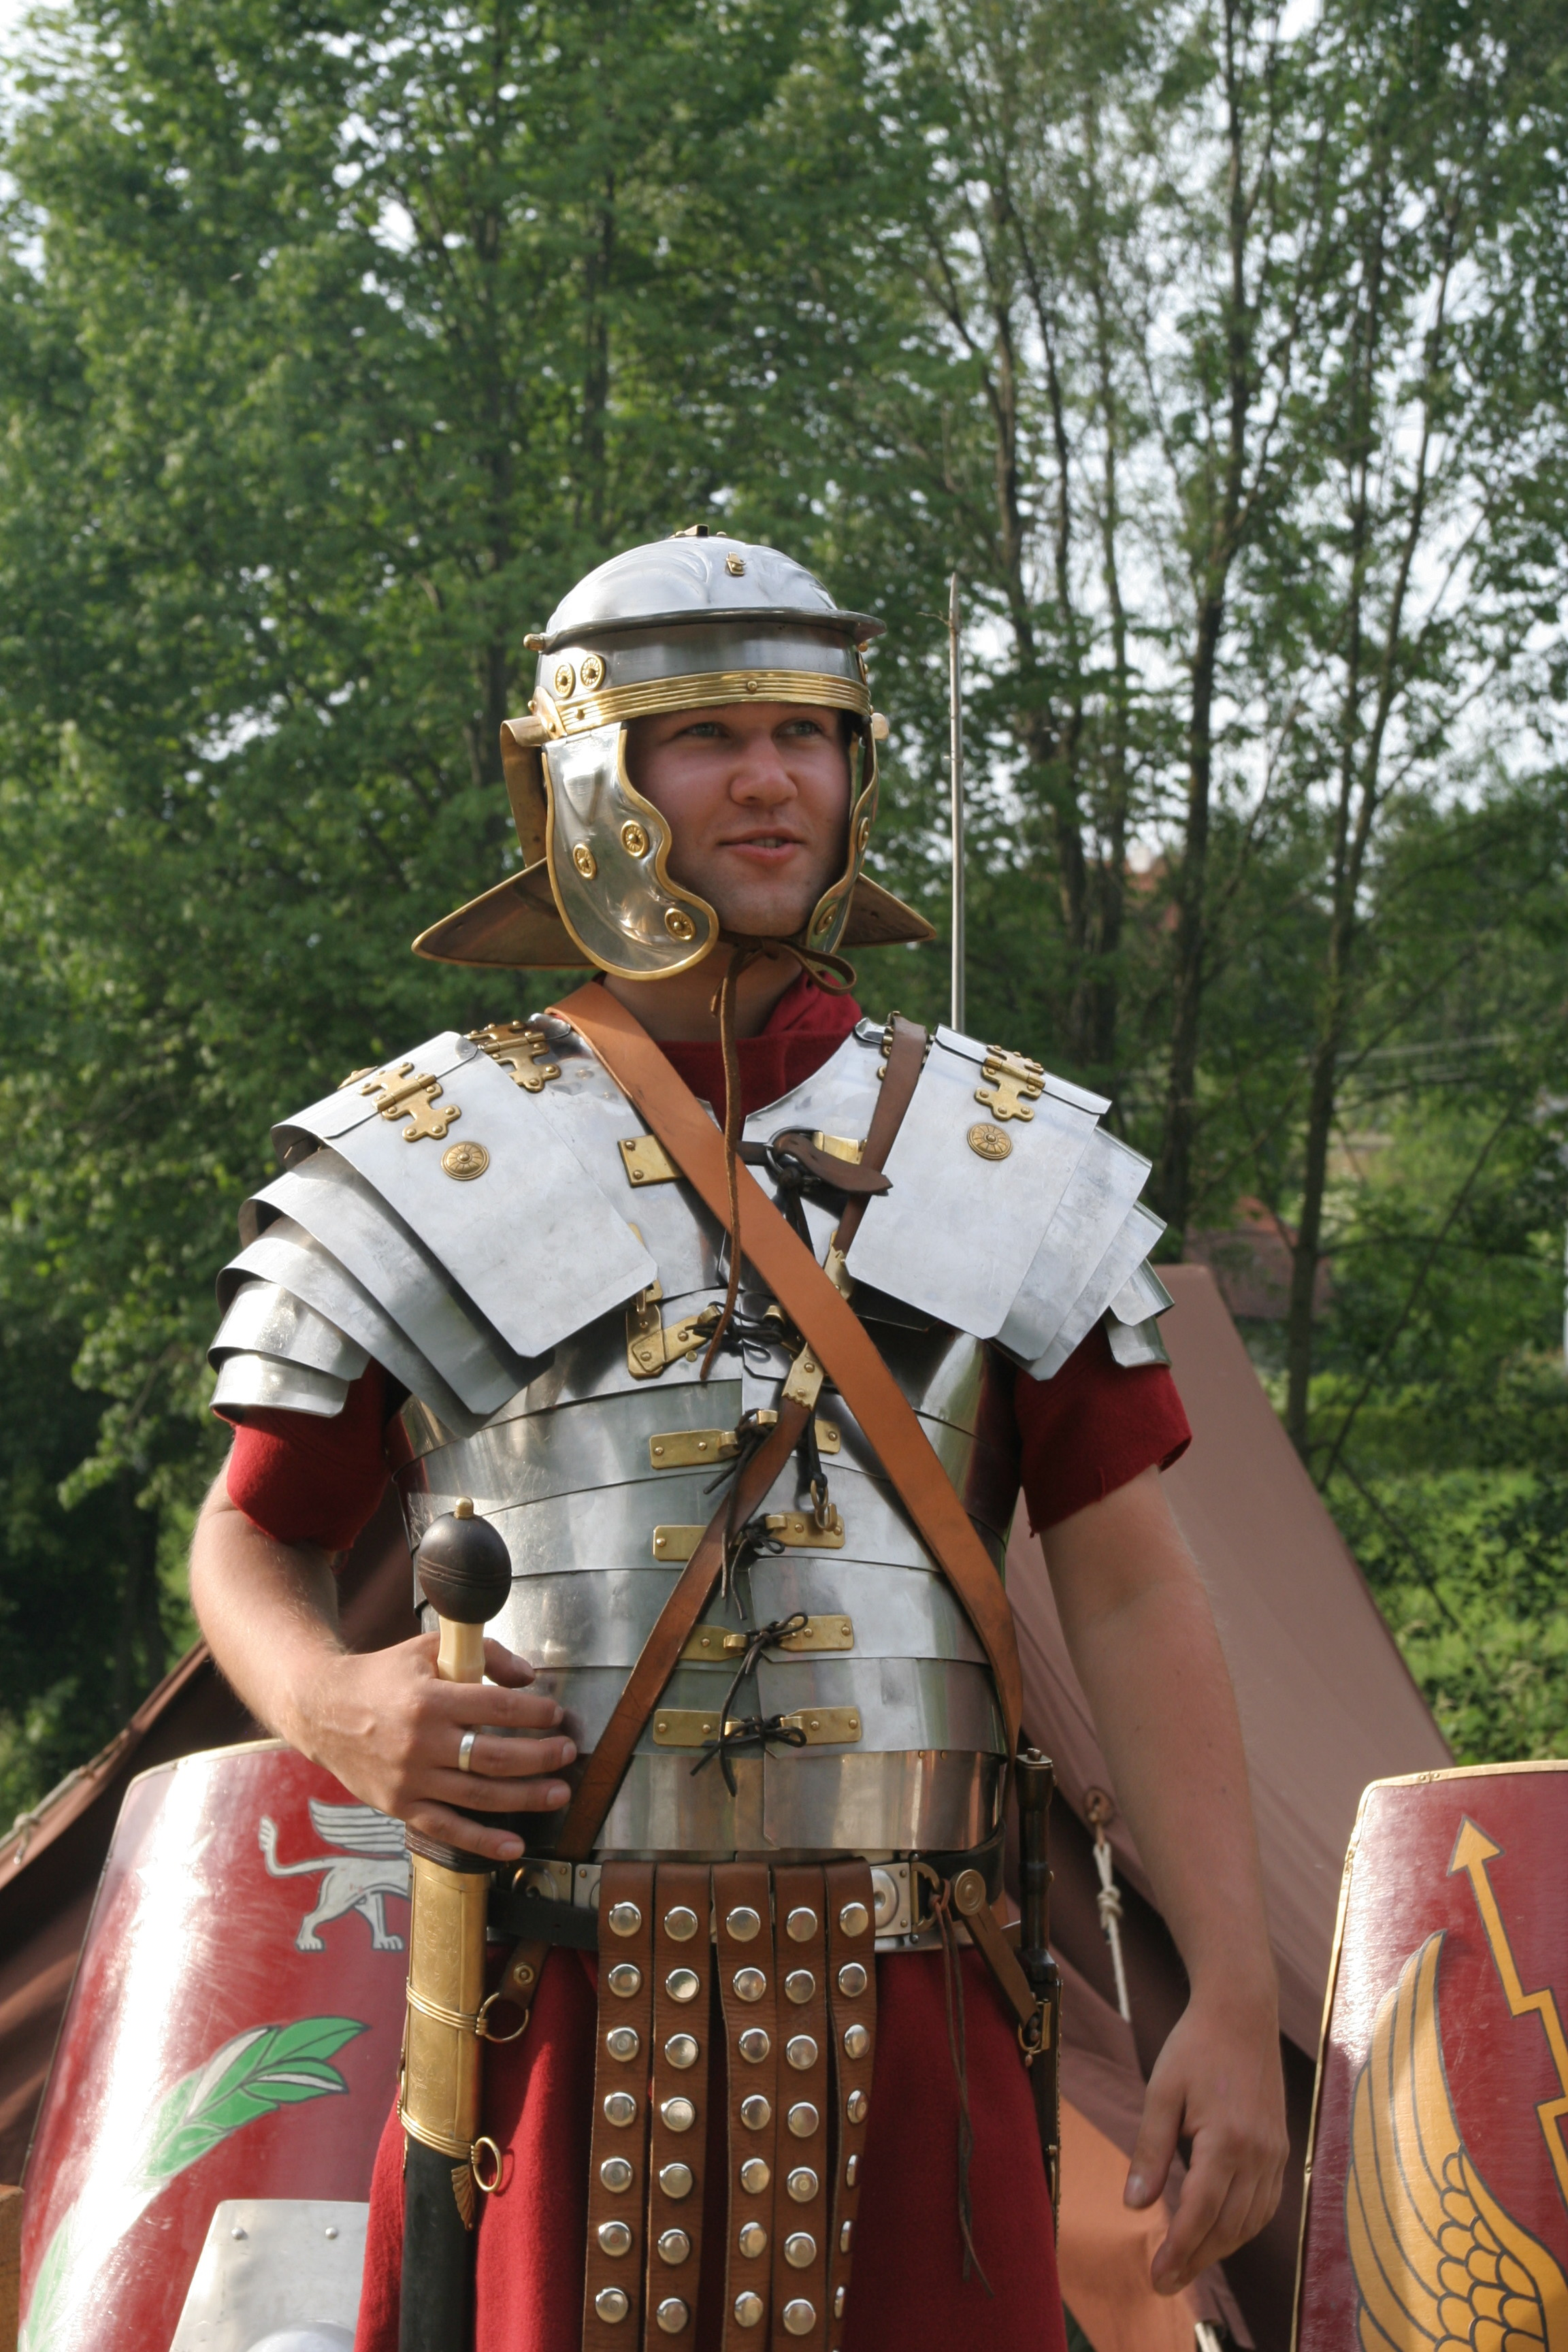
\includegraphics[width=0.42\paperwidth]{../ressources/Roman_soldier}
	\caption{Uniforme d'un légionnaire romain du \siecle{1} siècle. \cite{infantery}}
	\end{centering}
\end{figure}
\begin{figure}[H]
	\begin{centering}
	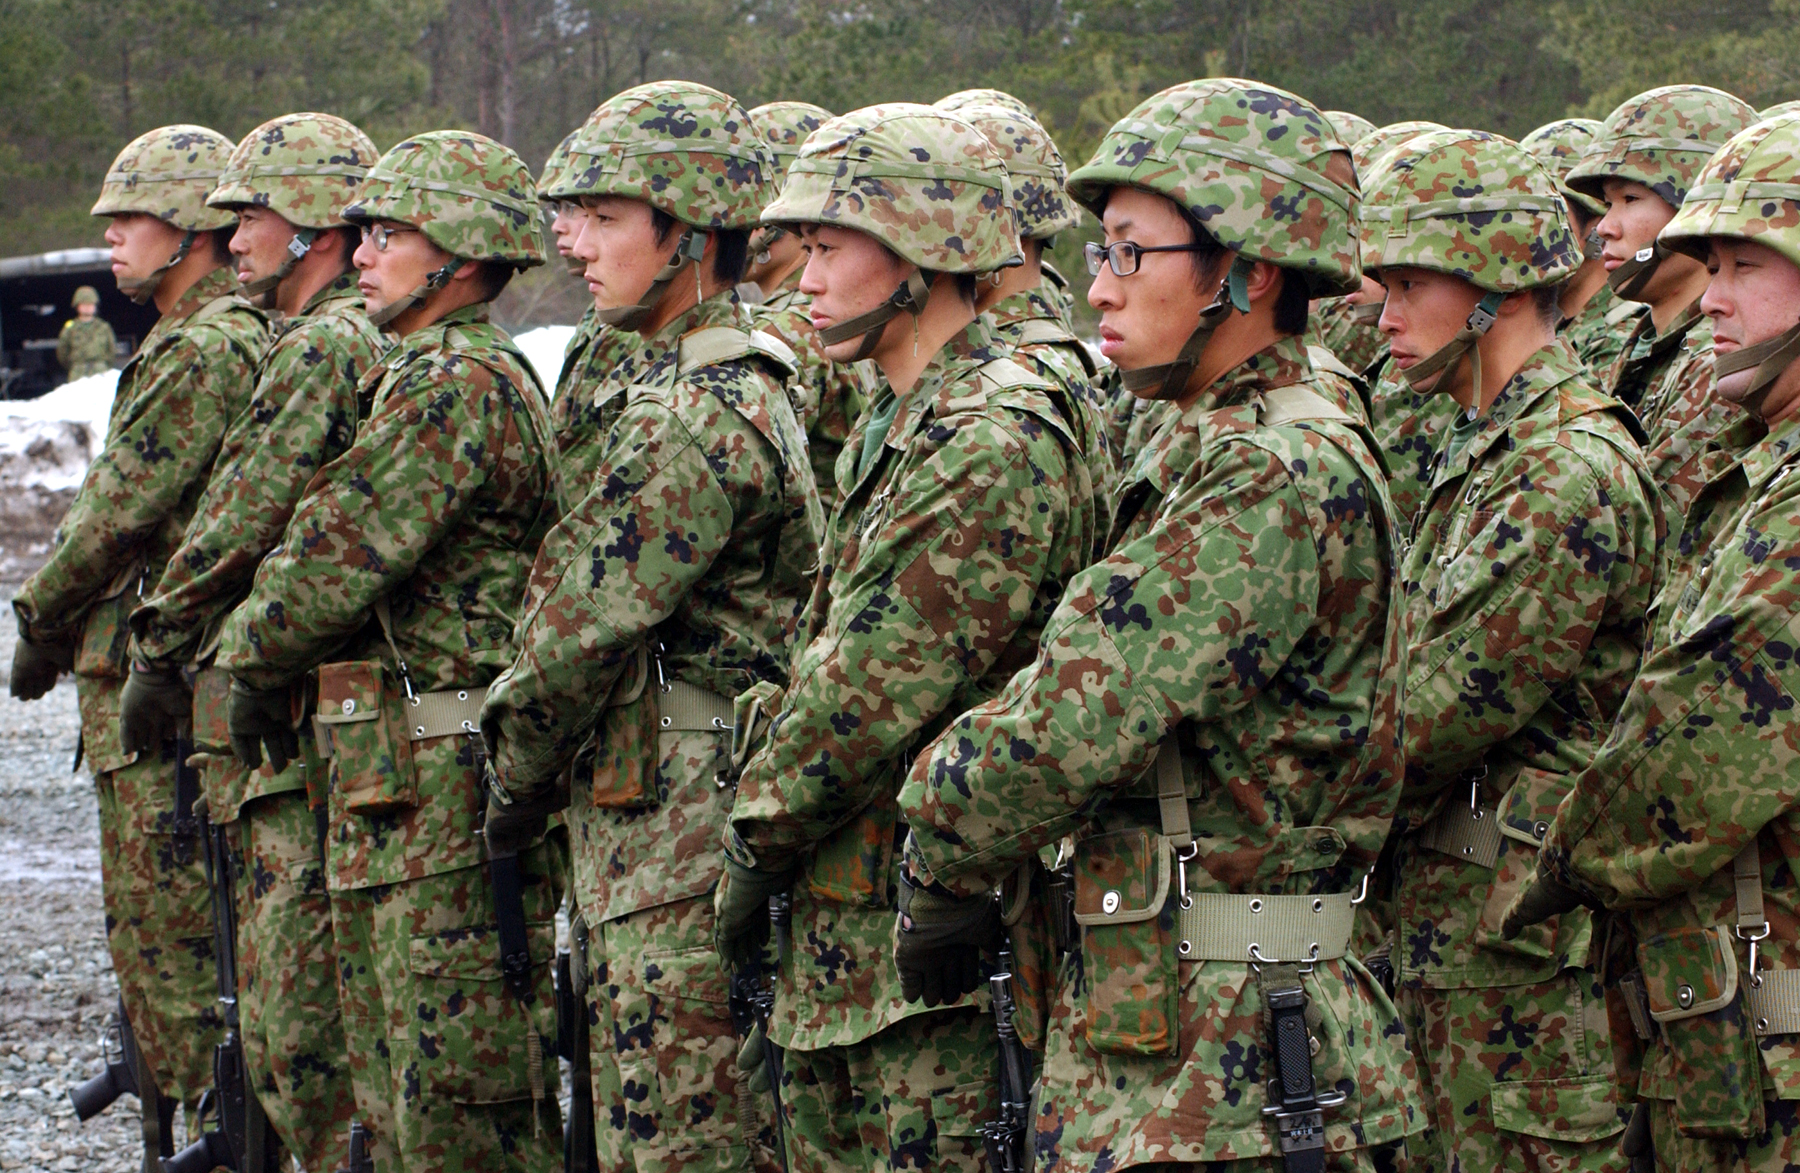
\includegraphics[width=0.55\paperwidth]{../ressources/JGDSF_Soldiers}
	\caption{Japan Ground Self-Defense Force infantry. \cite{infantery}}
	\end{centering}
\end{figure}

\subsubsection{Cavalerie légère}
\begin{figure}[H]
	\begin{centering}
	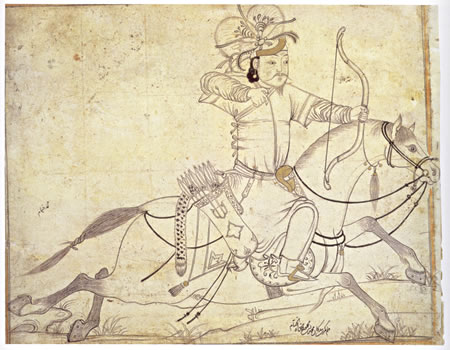
\includegraphics[width=0.5\paperwidth]{../ressources/IlkhanidHorseArcher}
	\caption{Archer à cheval Houlagides. \cite{archery}}
	\end{centering}
\end{figure}
\begin{figure}[H]
	\begin{centering}
	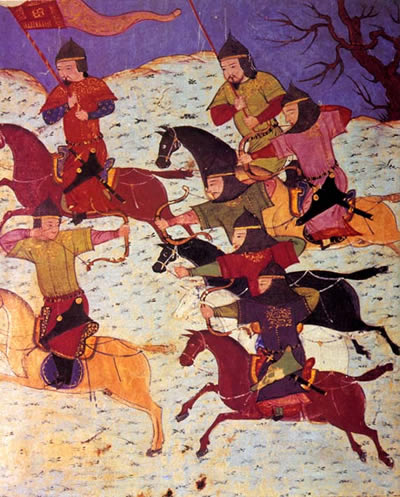
\includegraphics[width=0.47\paperwidth]{../ressources/MongolCavalrymen}
	\caption{Archers mongoles à cheval au combat (illustration d'un manuscrit du début du xive siècle) \cite{mongol_army}}
	\end{centering}
\end{figure}


\subsubsection{Cavalerie lourde}
\begin{figure}[H]
	\begin{centering}
	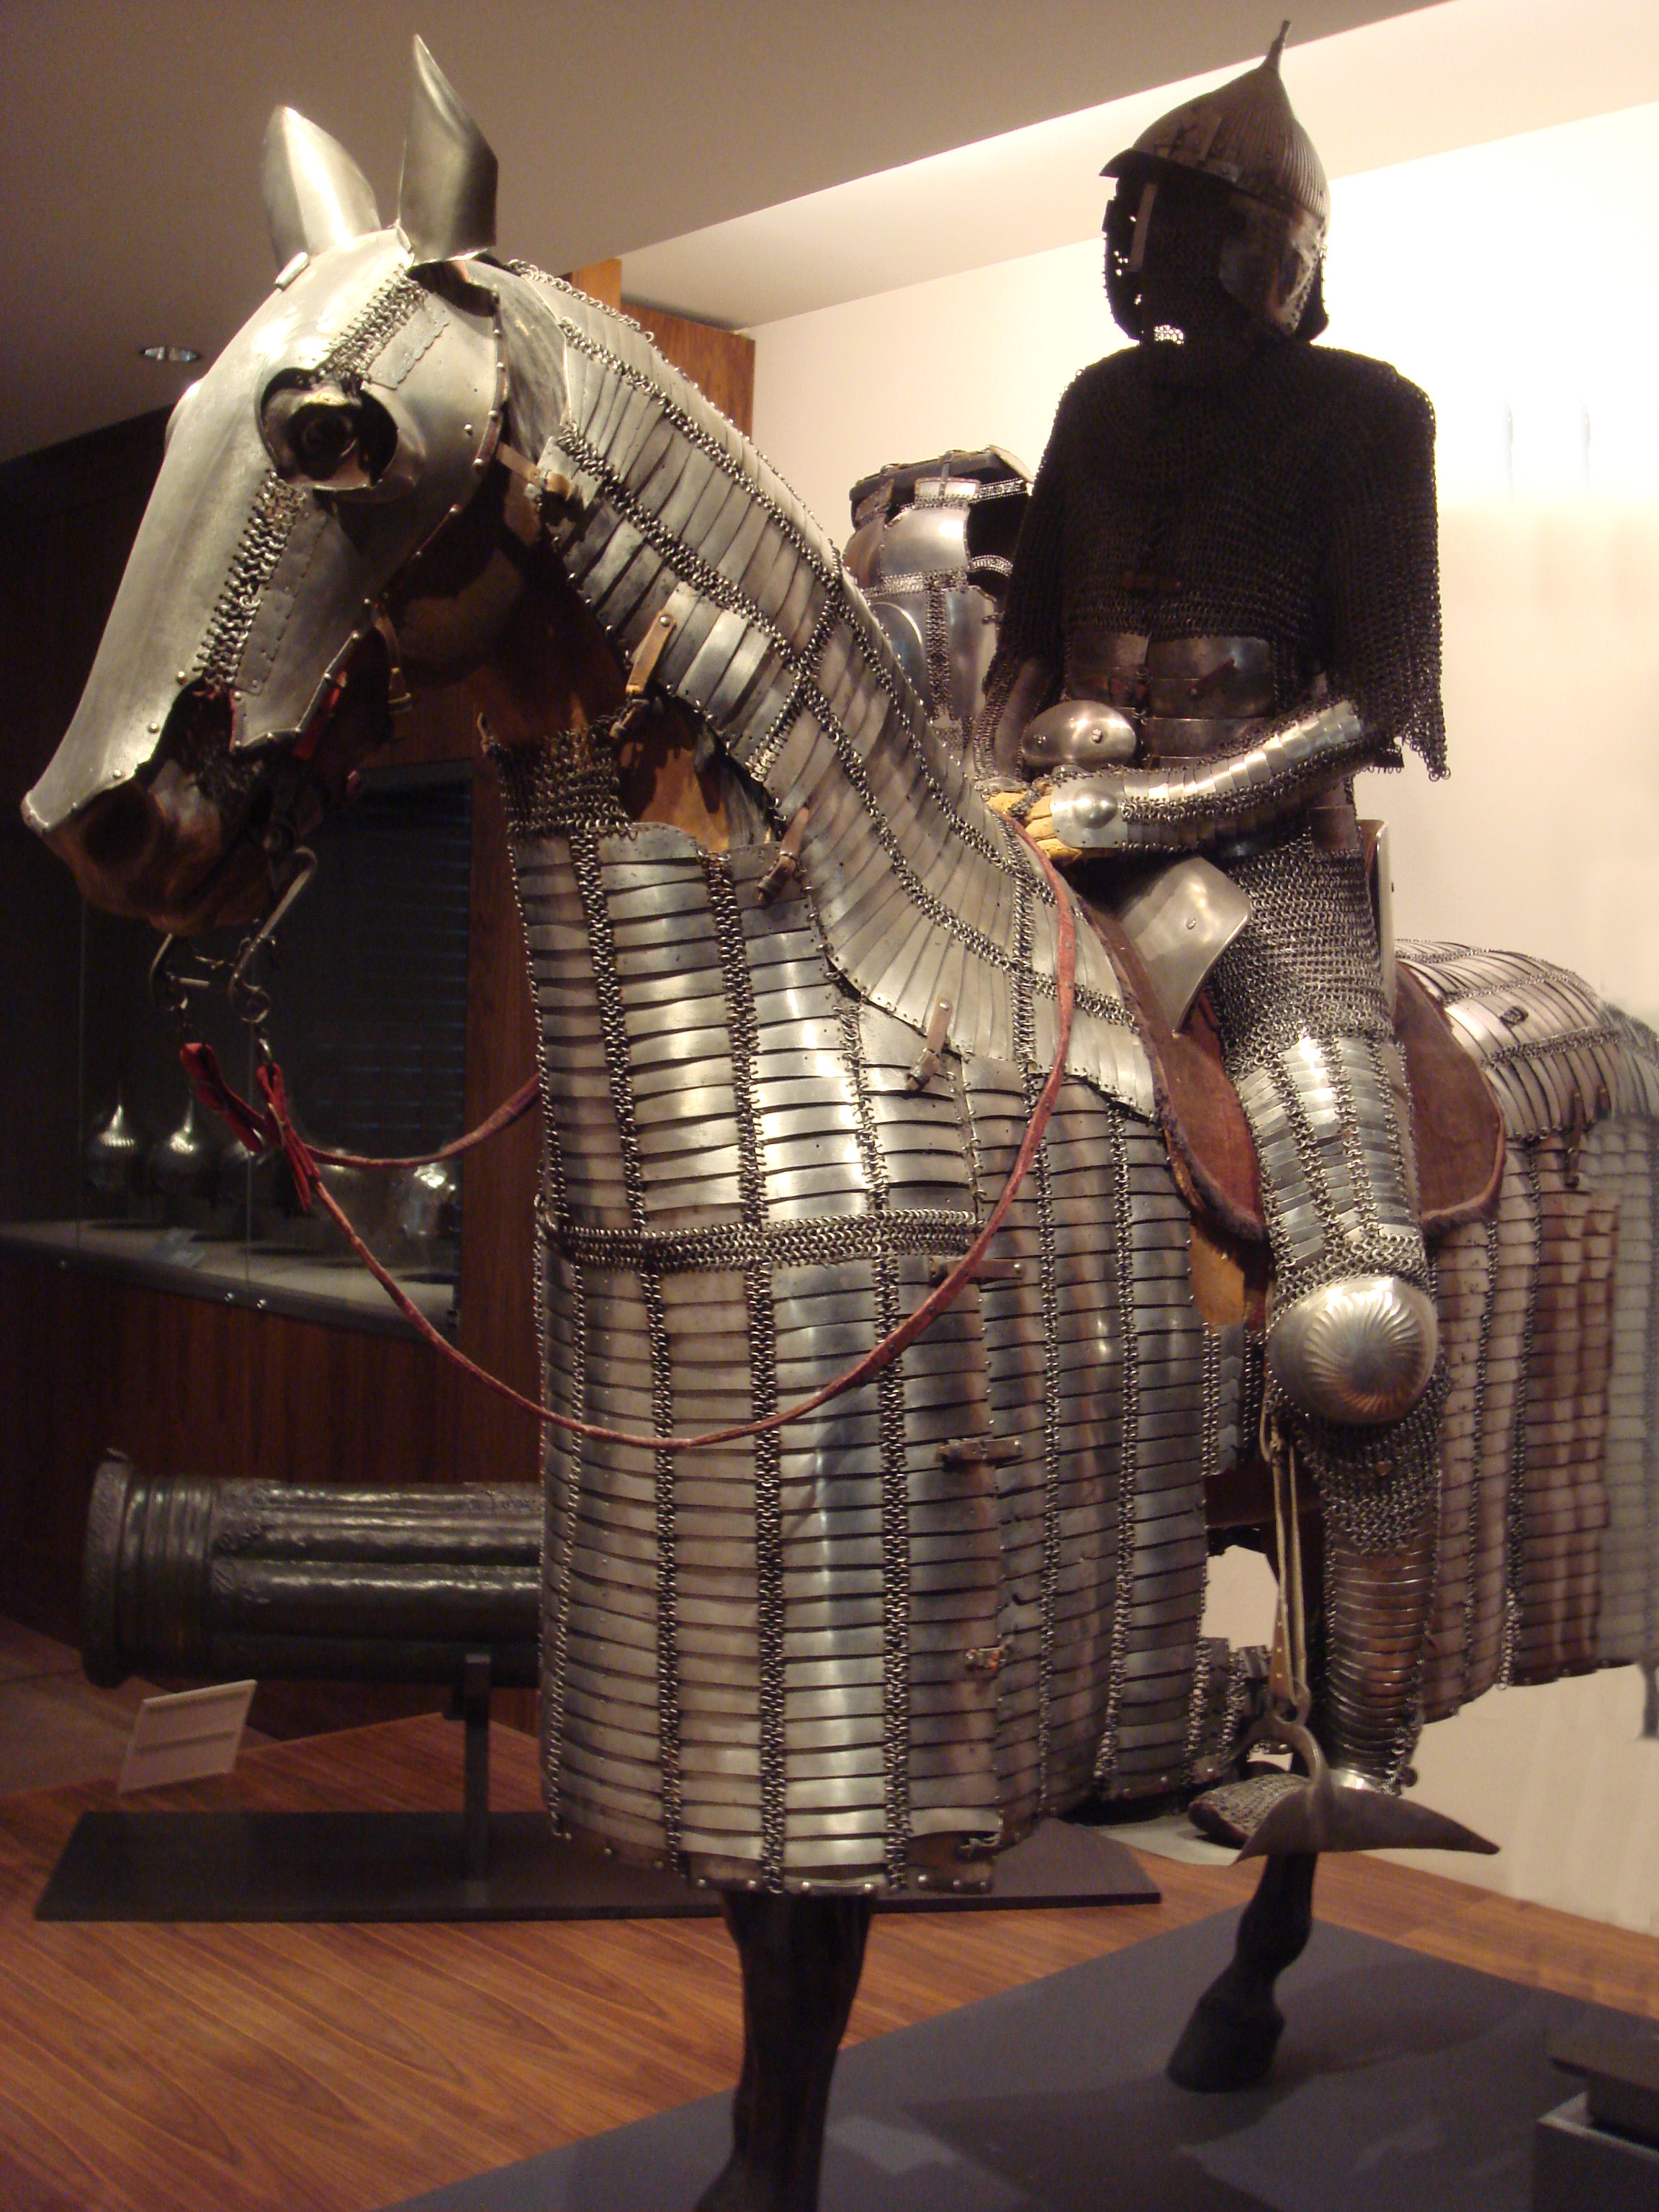
\includegraphics[width=0.44\paperwidth]{../ressources/Ottoman_Mamluk_horseman}
	\caption{Ottoman Mamluk heavy cavalry, circa 1550. \cite{heavy_cavalry}}
	\end{centering}
\end{figure}
\begin{figure}[H]
	\begin{centering}
	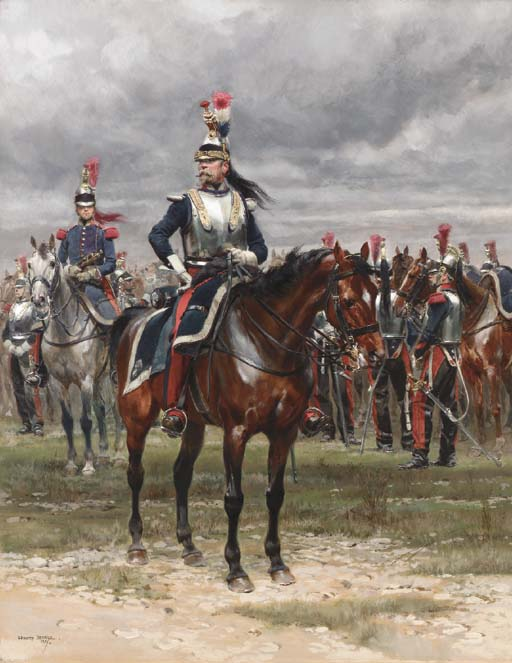
\includegraphics[width=0.5\paperwidth]{../ressources/cuirassiers}
	\caption{French cuirassiers, 19th century \cite{heavy_cavalry}}
	\end{centering}
\end{figure}

\subsubsection{Formation en triple ligne}
\begin{figure}[H]
	\begin{centering}
	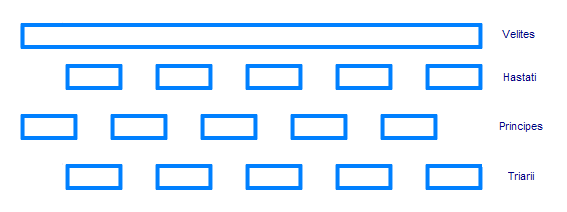
\includegraphics[width=\linewidth]{../ressources/Polybian_formation}
	\caption{Disposition classique en trois lignes \cite{roman_infantry_tactics}}
	\end{centering}
\end{figure}
\begin{figure}[H]
	\begin{centering}
	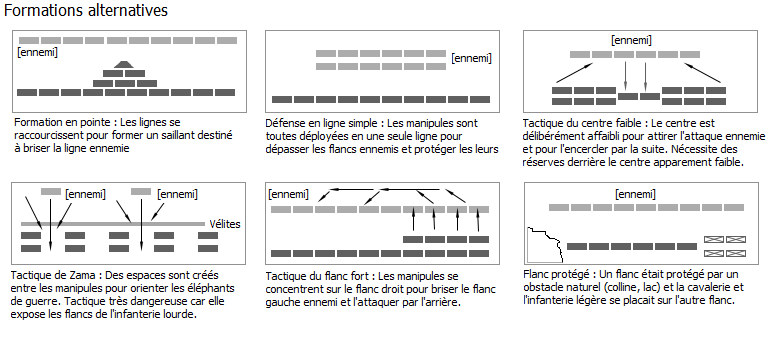
\includegraphics[width=\linewidth]{../ressources/Formations_infanterie_romaine}
	\caption{Formations alternatives \cite{roman_infantry_tactics}}
	\end{centering}
\end{figure}



\subsection{Tactiques}

\subsubsection{Charge}
\begin{figure}[H]
	\begin{centering}
	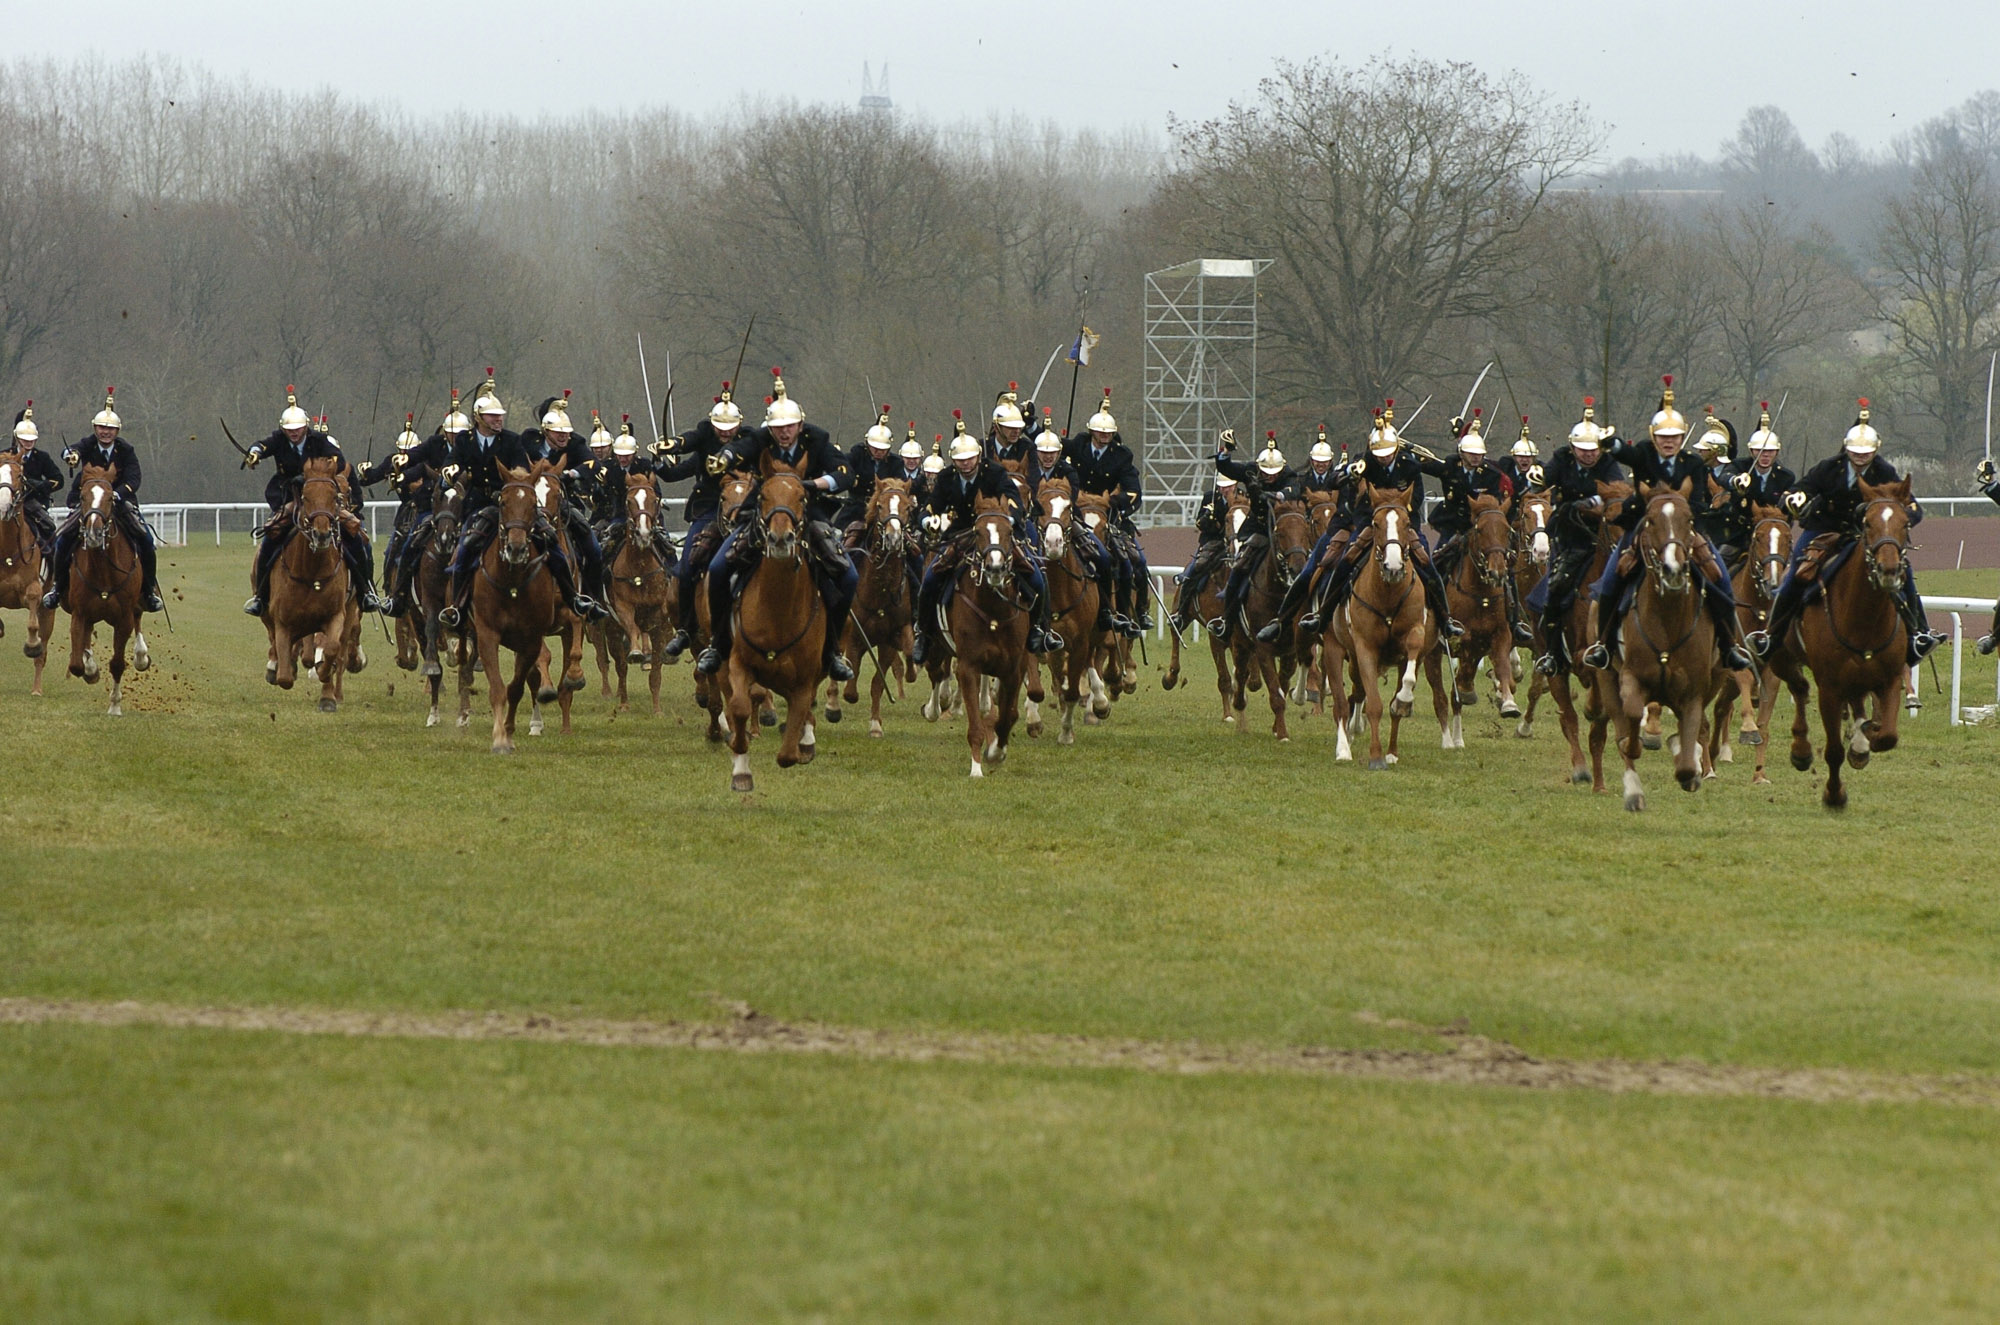
\includegraphics[width=\linewidth]{../ressources/Charge-de-cavalerie}
	\caption{Charge de cavalerie de la garde républicaine \cite{charge_cavalery}}
	\end{centering}
\end{figure}
\begin{figure}[H]
	\begin{centering}
	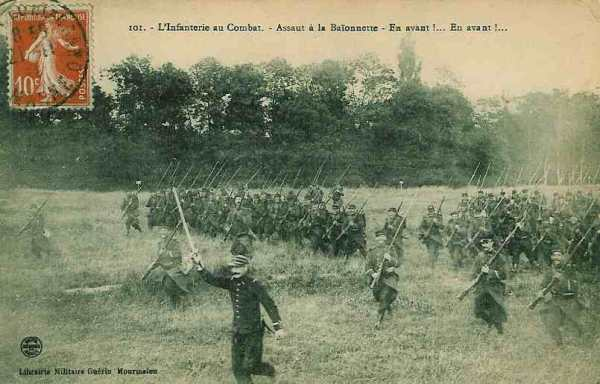
\includegraphics[width=\linewidth]{../ressources/charge_infanterie}
	\caption{Charge d’infanterie française 1914 \cite{infantery_charge}}
	\end{centering}
\end{figure}
\cite{charge_tactic}

\subsubsection{Manœuvre de flanquement}
\begin{figure}[H]
	\begin{centering}
	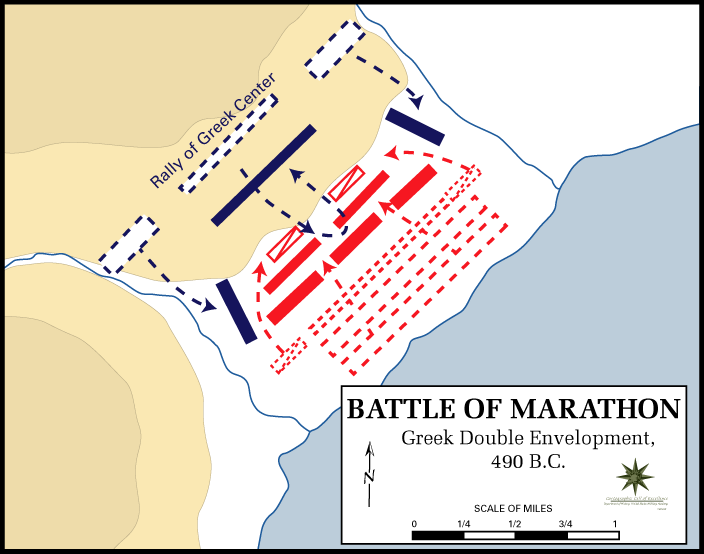
\includegraphics[width=\linewidth]{../ressources/Battle_of_Marathon}
	\caption{Bataille de Marathon (double enveloppement, manœuvre de flanquement) \cite{flanking_maneuver}}
	\end{centering}
\end{figure}
\begin{figure}[H]
	\begin{centering}
	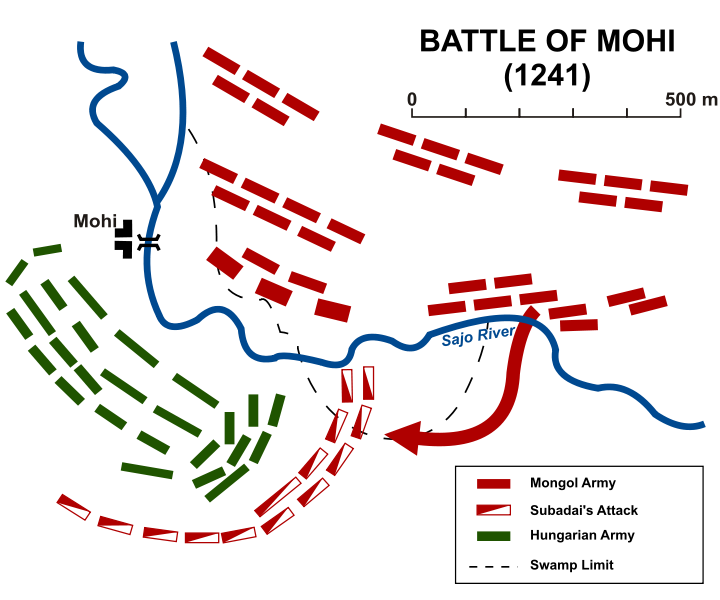
\includegraphics[width=\linewidth]{../ressources/Battle_of_Mohi}
	\caption{Plan de la bataille de Mohi (Hongrie) \cite{mohi_battle}}
	\end{centering}
\end{figure}
\cite{tactic,pincer_tactic}

\subsubsection{Le marteau et l'enclume}
\begin{figure}[H]
	\begin{centering}
	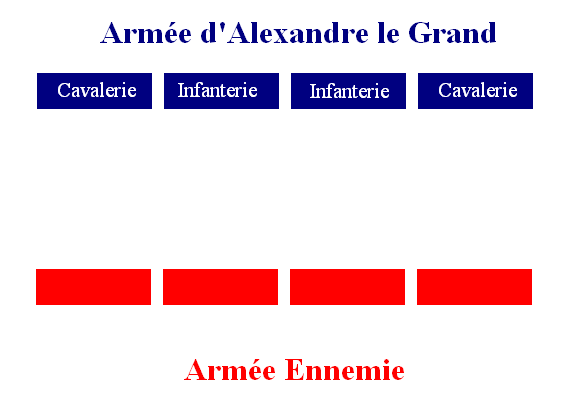
\includegraphics[width=0.8\linewidth]{../ressources/marteau}
	\caption{}
	\end{centering}
\end{figure}
\begin{figure}[H]
	\begin{centering}
	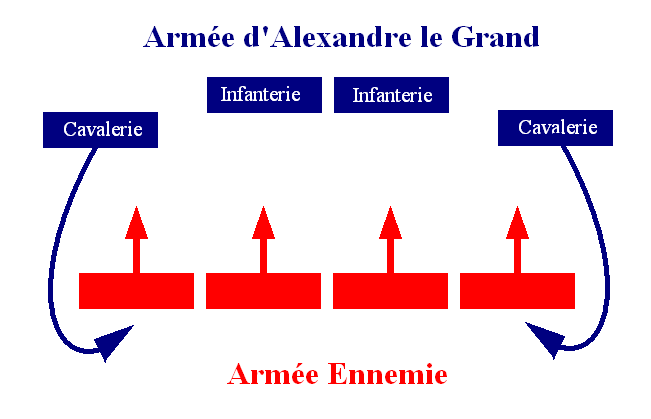
\includegraphics[width=0.8\linewidth]{../ressources/marteau2}
	\caption{}
	\end{centering}
\end{figure}
\begin{figure}[H]
	\begin{centering}
	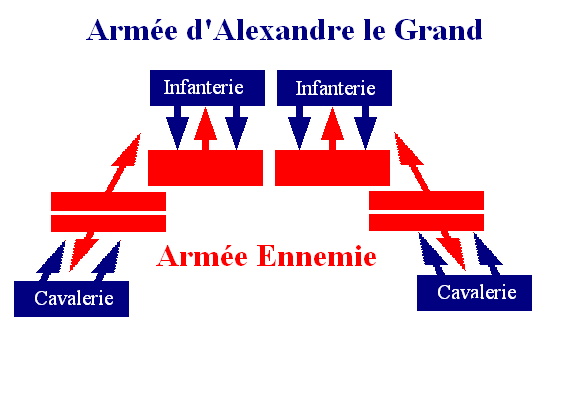
\includegraphics[width=0.8\linewidth]{../ressources/enclume}
	\caption{}
	\end{centering}
\end{figure}
\begin{figure}[H]
	\begin{centering}
	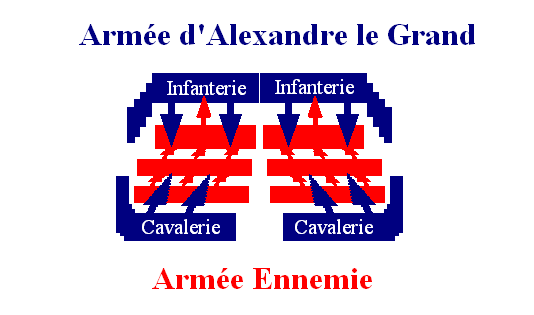
\includegraphics[width=0.8\linewidth]{../ressources/enclume2}
	\caption{}
	\end{centering}
\end{figure}
\cite{Alexanders_tactics}

\subsubsection{Contre-attaque}
\begin{figure}[H]
	\begin{centering}
	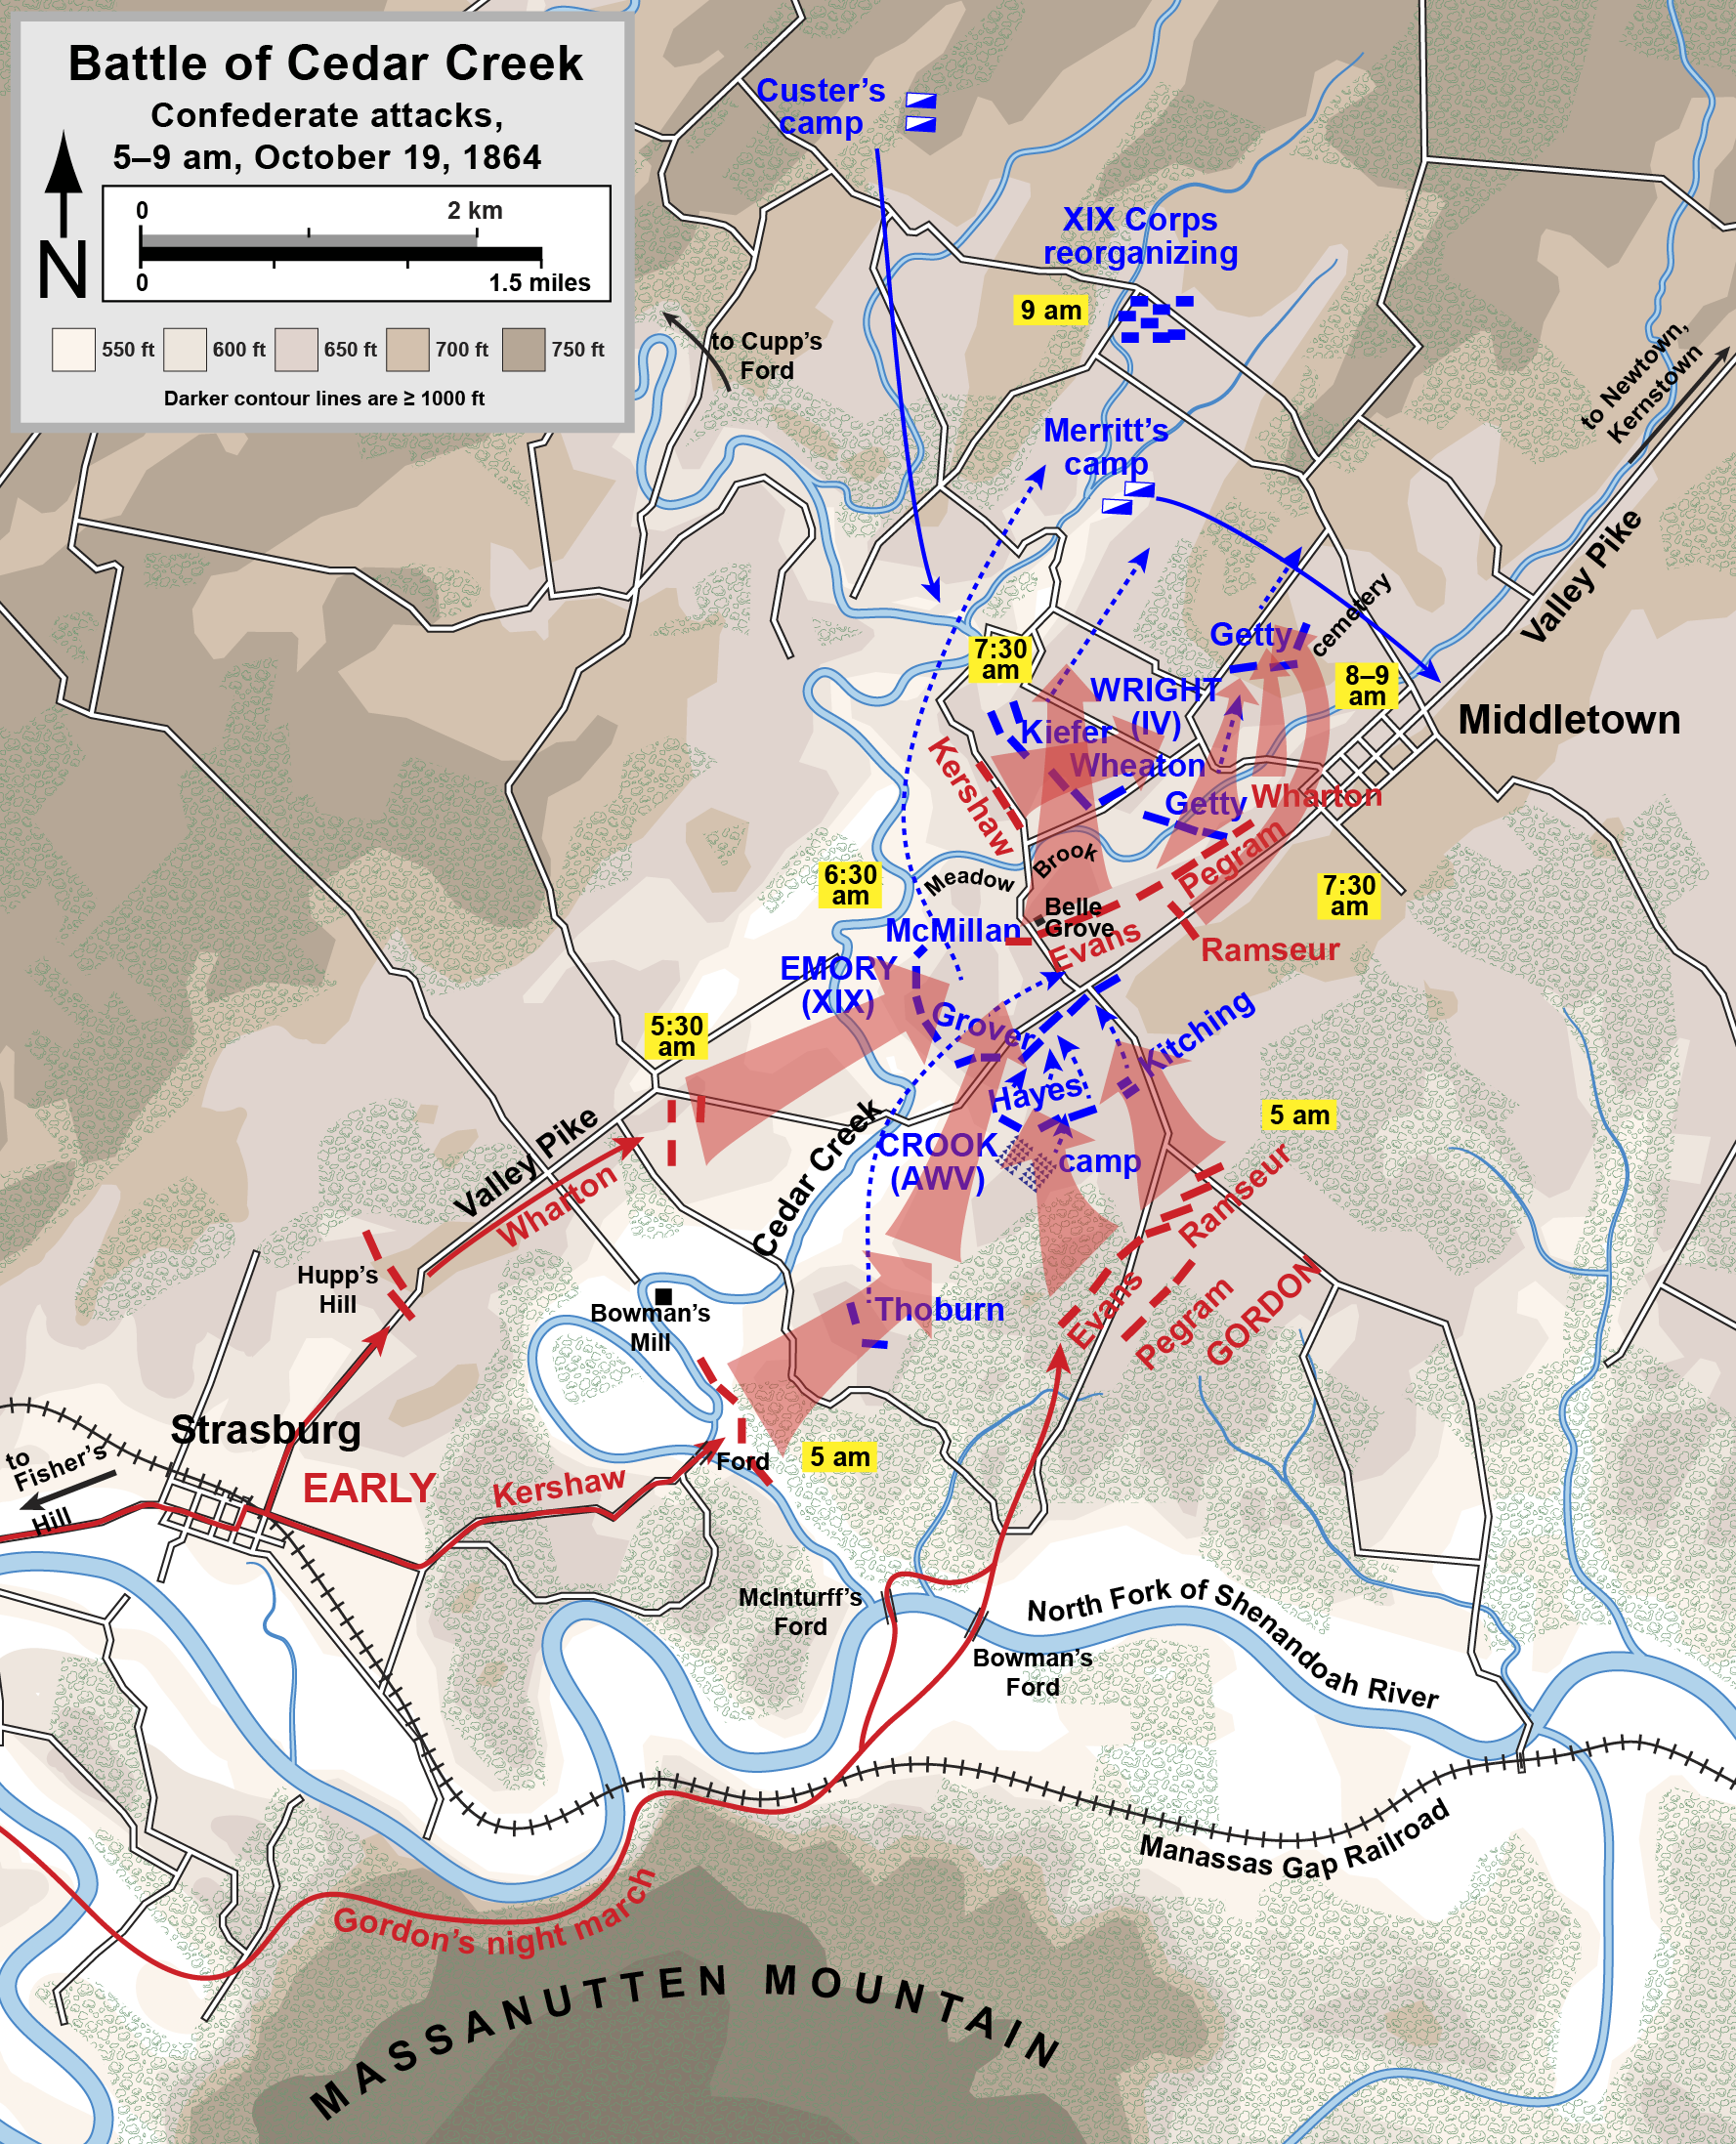
\includegraphics[width=\linewidth]{../ressources/Cedar_Creek_Confederate_attacks}
	\caption{Battle of Cedar Creek, Confederate attacks}
	\end{centering}
\end{figure}
\begin{figure}[H]
	\begin{centering}
	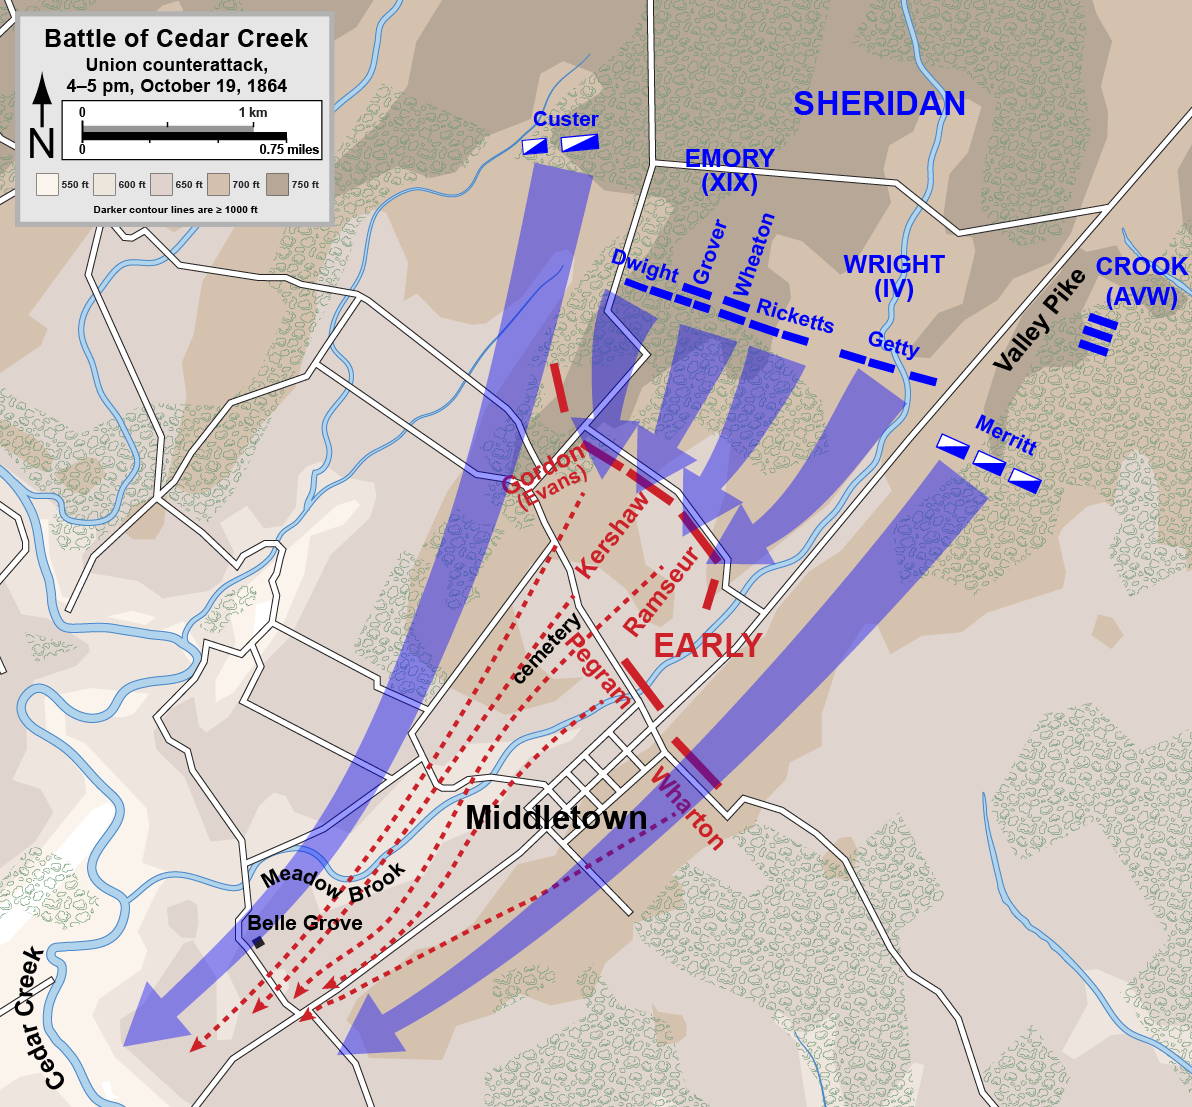
\includegraphics[width=\linewidth]{../ressources/Cedar_Creek_Union_counterattack}
	\caption{Battle of Cedar Creek, Union counterattack}
	\end{centering}
\end{figure}
\cite{counterattack_wiki, couterattack_cedar_creek}

\subsubsection{Retraite feinte}
\begin{figure}[H]
	\begin{centering}
	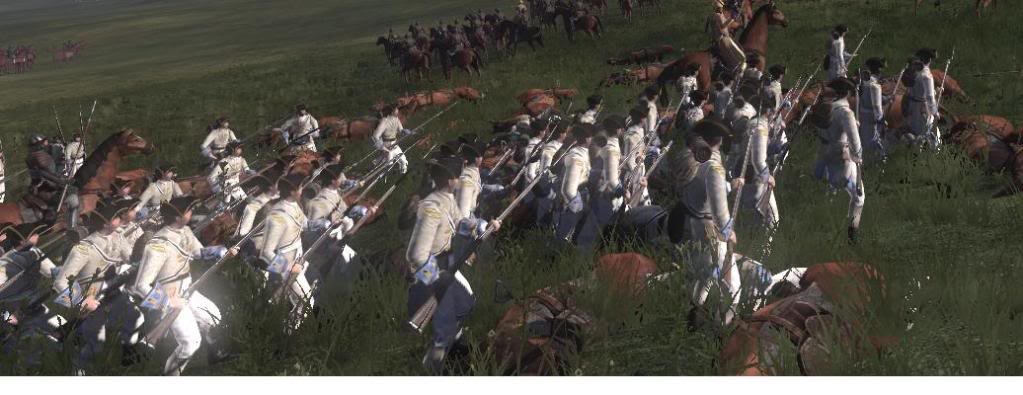
\includegraphics[width=\linewidth]{../ressources/infantrysquare3}
	\caption{These French troops broke formation, and are pursuing the enemy cavalry. \cite{feigned_retreat}}
	\end{centering}
\end{figure}
\cite{mongol_army}


\subsubsection{Embuscade}
\begin{figure}[H]
	\begin{centering}
	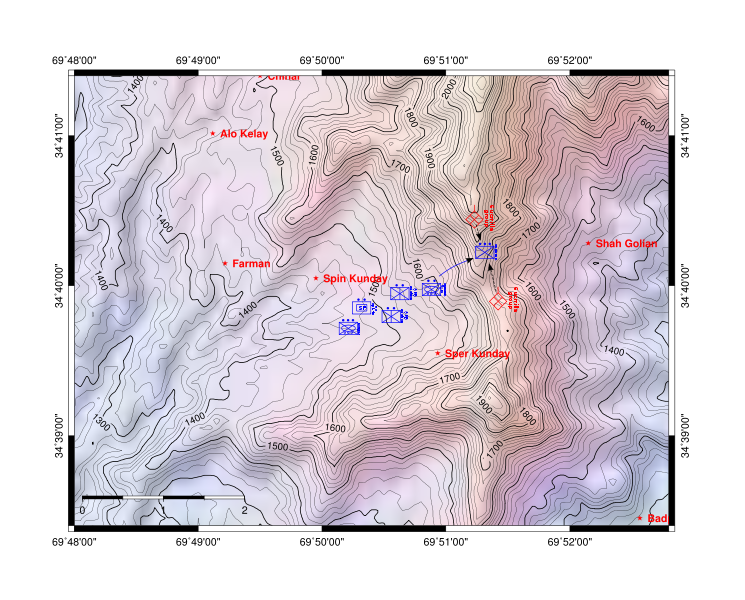
\includegraphics[width=\linewidth]{../ressources/Uzbin_valley_ambush-map}
	\caption{Embuscade d'Uzbin \cite{uzbin_ambush}}
	\end{centering}
\end{figure}
\begin{figure}[H]
	\begin{centering}
	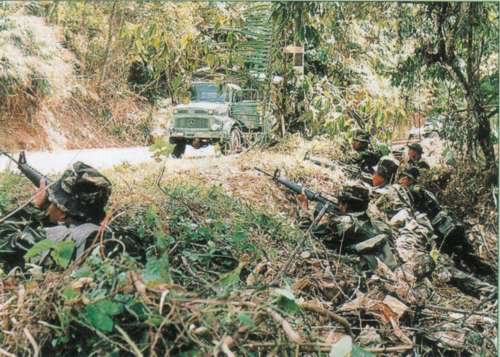
\includegraphics[width=0.8\linewidth]{../ressources/ambush}
	\caption{Malaysian Armed Forces ambush \cite{ambush_picture}}
	\end{centering}
\end{figure}
\cite{ambush_wiki}

\subsubsection{Hit and run}




\section{Applications aux systèmes multi-agents}

\subsection{Enhanced Isaac Neural Simulation Toolkit (EINSTein)}
%http://wwwhome.ewi.utwente.nl/~hmiproj6/AL/isaac_einstein_paper.pdf
%https://hmi.ewi.utwente.nl/~hmiproj6/AL/mors.pdf
%http://en.wikipedia.org/wiki/Braitenberg_vehicle
%http://en.wikipedia.org/wiki/Lanchester's_laws
%http://www2.dcs.hull.ac.uk/NEAT/dnd/AI/AndyIlachinski_BriefingSlides.pdf

\subsubsection{Origines}
\textbf{EINSTein} (\underline{E}nhanced \underline{I}SAAC \underline{N}eural \underline{S}imulation \underline{T}oolkit), conçu sous Andy Ilachinksi en 1999, se présente comme \og{}laboratoire\fg{} de vie artificielle, fut implémenté dans le but de faciliter l'exploration de l'auto-orgnisation et l'emmergence dans le combat terrestre. 

\begin{center}
\begin{figure}[H]
\begin{minipage}[H]{0.25\linewidth}
	\centering
	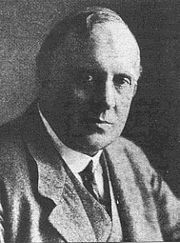
\includegraphics[width=\textwidth]{../ressources/lanchester}
	\caption{Frederick W. Lanchester}
\end{minipage}
\hfill
\begin{minipage}[H]{0.25\linewidth}
	\centering
	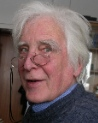
\includegraphics[width=\textwidth]{../ressources/valentin_braitenberg}
	\caption{Valentin Braintenberg}
\end{minipage}
\hfill
\begin{minipage}[H]{0.25\linewidth}
	\centering
	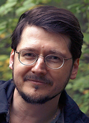
\includegraphics[width=\textwidth]{../ressources/ilachinski}
	\caption{Andy Ilachinski}
\end{minipage}
\end{figure}
\end{center}

Il se base sur \textbf{ISAAC}(\underline{I}rreducible \underline{S}emi-\underline{A}utonomus \underline{A}daptive \underline{C}ombat)~: modèle crée par opposition à la vision réductioniste et par le haut des Lois de Lanchester, formules utilisés couramment pour modéliser l'attrition depuis 1916. ISAAC se base d'ailleurs lui-même sur les \og{}Vehicles\fg{} de Valentino Braitenberg, agents munis de senseurs et possèdant des effecteurs leur permettant de se déplacer dans leur environnement. Si les Vehicles apportent la notion de \emph{multum in parvo} et ISAAC applique cette vision synthesiste et par le bas à la modélisation du combat terrestre, EINSTein étend, ameliore et concrétise sa preuve de concept, et l'encapsule dans une boite à outils pour développeurs.

\subsubsection{Fonctionnement}

\begin{center}
\begin{figure}[H]
	\begin{centering}
	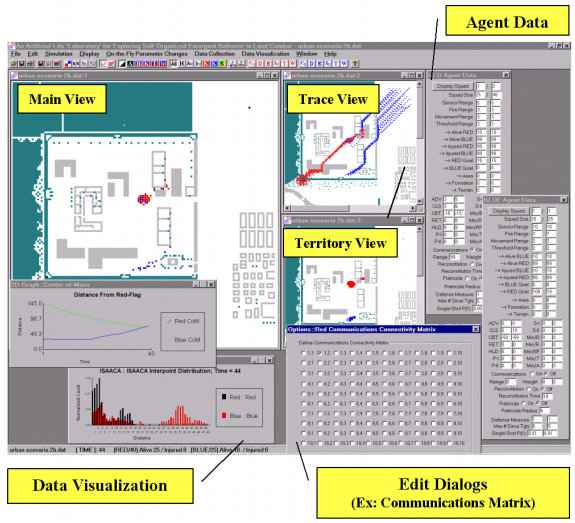
\includegraphics[width=0.9\linewidth]{../ressources/Einstein}
	\caption{Interface développé pour EINSTein}
	\end{centering}
\end{figure}
\cite{simu_guerre,ilachinski1994,ilachinski1999}
\end{center}

Un ensemble d'automates cellulaires mobiles divisés en deux équipes se confrontent, le but étant pour chaque équipe d'atteindre le drapeau de l'autre sans que le sien soit touché. Chaque agent dispose d'une personalité~: un ensemble de ponderations pour chaque percept possible (enemies ou alliés sains ou bléssés, drapeaux, etc) différent pour chaque état. L'agent aura donc plus ou moins envie d'approcher la source d'un percept selon sa personalité et son état physique.

\begin{center}
\begin{figure}[H]
\begin{minipage}[H]{0.35\linewidth}
	\centering
	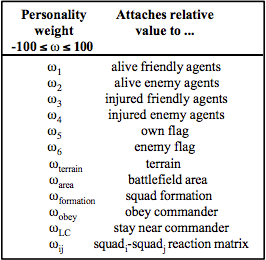
\includegraphics[width=\textwidth]{../ressources/einstein_personality_weight}
\end{minipage}
\hfill
\begin{minipage}[H]{0.55\linewidth}
	\centering
	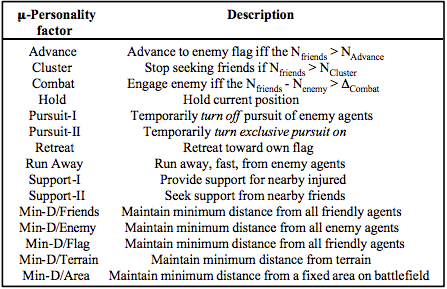
\includegraphics[width=\textwidth]{../ressources/einstein_personality_factor}
\end{minipage}
\caption{Agent EINSTein~: ponderations de comportements et meta-règles}
\end{figure}
\end{center}

En plus de sa personalité, un ensemble de \og{}meta-règles\fg{} influencent ses décisions. Il aura par exemple envie d'avancer vers le drapeau enemie, mais ne le fera pas sans qu'il ait atour de lui un certain nombre d'alliés.

\begin{figure}[H]
	\begin{center}
	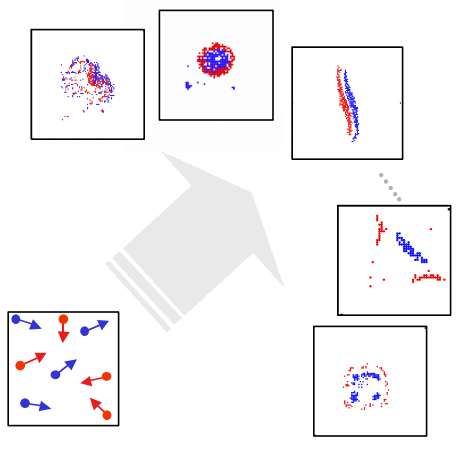
\includegraphics[width=0.8\linewidth]{../ressources/einstein_global_behavior}
	\caption{Tactiques emmergeants retrouvés dans ISAAC et EINSTein}
	\end{center}
\end{figure}

Avec cet architecture simple et un peu d'apprentissage automatique par algorithmes génétiques, nous arrivons à des tactiques intéressantes tels formations en pointe, encerclement, prises en ténaille, attaques guérilla,~\dots

\subsection{Iruba}

\begin{wrapfigure}{r}{0.3\textwidth}
  \begin{center}
	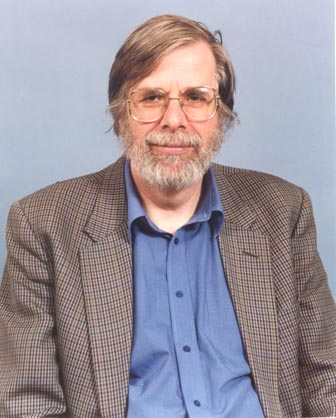
\includegraphics[width=0.2\textwidth]{../ressources/doran}
	\caption{Jim Doran}
  \end{center}
\end{wrapfigure}

An Agent-Based Model of the Guerrilla War Process 2005.


\begin{figure}[H]
	\begin{centering}
	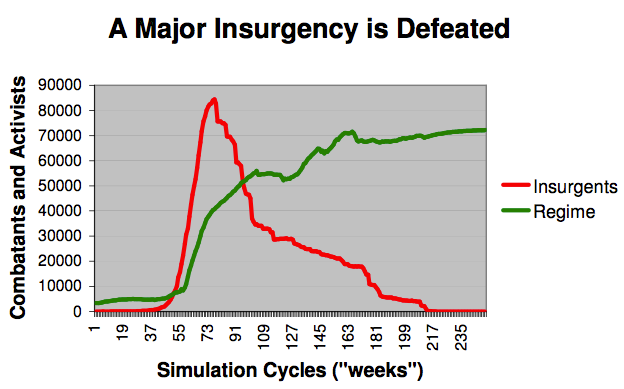
\includegraphics[width=\linewidth]{../ressources/insurgency}
	\end{centering}
\end{figure}
\begin{algorithmic}[1]
		\WHILE{non termination}
			\STATE Attacks and their impact
			\STATE HQ decisions
			\STATE Recruitment
			\STATE Force movement
		\ENDWHILE
		\end{algorithmic}
\cite{doran2005iruba}

Stratégies influant sur la réussite
initial guerrilla band size
regime force concentration
insurgent mobility
insurgent hyper-mobility
all-out regime counter attack

\begin{center}
\begin{figure}[H]
\begin{minipage}[H]{0.4\linewidth}
	\centering
	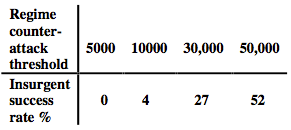
\includegraphics[width=\linewidth]{../ressources/iruba_counter_attack}
\end{minipage}
\hfill
\begin{minipage}[H]{0.4\linewidth}
	\centering
	\includegraphics[width=\linewidth]{../ressources/iruba_force_concentration}
\end{minipage}
\end{figure}
\begin{figure}[H]
\begin{minipage}[H]{0.4\linewidth}
	\centering
	\includegraphics[width=0.9\linewidth]{../ressources/iruba_hyper_mobility}
\end{minipage}
\hfill
\begin{minipage}[H]{0.4\linewidth}
	\centering
	\includegraphics[width=\linewidth]{../ressources/iruba_mobility}
\end{minipage}
\caption{Stratégies influant sur la réussite des agents Iruba}
\end{figure}
\end{center}

\subsection{RPDAgent (Recogition-Primed Decision Agent)}
% http://en.wikipedia.org/wiki/Recognition_primed_decision
\subsubsection{Recognition-primed Decision model}
Developpé par Gary Klein à partir de 1985, le modèle RPD (\underline{R}ecognition-\underline{P}rimed \underline{D}ecision) est un modèle théorique qui vise à décrire la manière dans lequel les êtres humains font des décisions. RPD s'inscrit dans le framework NDM (\underline{N}aturalistic \underline{D}ecision \underline{M}aking), qui s'oppose à l'agent rationnel comme modèle du décideur humain.
Un agent RPD base ses décisions sur d'une part une reconaissance de motifs et de l'autre sur un moteur de simulation~: deux mécanismes sont développés et renforcés à partir des expériences passées. Un agent RPD ne fait pas une énumeration des action possible mais prends plutôt la première action qui semblerait adéquat d'après ce qu'il a véçu. C'est donc un agent \og{}intuitive\fg{}.

\begin{figure}[H]
\centering
\begin{minipage}[H]{0.3\linewidth}
	\centering
	\includegraphics[width=\textwidth]{../ressources/klein}
	\caption{Gary Klein}
\end{minipage}
\hspace{0.1\linewidth}
\begin{minipage}[H]{0.3\linewidth}
	\centering
    \includegraphics[width=\textwidth]{../ressources/john_sokolowski}
    \caption{John A. Sokolowski}
\end{minipage}
\hfill
\end{figure}

\subsubsection{Travail de John Soklowski}
L'RPDAgent de Soklowski fut développé en 2003 dans le but de modéliser la prise de décision à grande échelle d'un générale humain. Notons que la problématique n'est pas de trouver une solution optimale, mais plutôt de passer un test de Turing, l'application visé étant celui de fournir de simuler un adversaire réaliste lors d'un entrainement et non pas de créer une machine capable de mener des vraies opérations militaires.
\begin{figure}[H]
\centering
\begin{minipage}[H]{0.4\linewidth}
	\centering
	\includegraphics[width=\textwidth]{../ressources/RPDagent_uml}
	\caption{Diagramme UML de l'agent composite RPDAgent}
\end{minipage}
\hfill
\begin{minipage}[H]{0.55\linewidth}
En pratique l'agent RPD est un agent composite formés de plusieurs sous-agents. Il reçoit soit des appels à la decision soit des appels de révision d'actions à base de nouvelles informations, et réagit ainsi~:
\begin{algorithmic}[1]
\STATE \emph{RecognitionAgent}: analyse situation
\STATE \emph{SymbolicConstructorAgent}: create internal representation
\FORALL {decisions}
\STATE new \emph{DecisionAgent}: consider this decision
\FORALL {goals}
\STATE new \emph{ReactiveAgent}: consider this goal wrt. this decision
\ENDFOR
\ENDFOR
\end{algorithmic}
Chaque \emph{ReactiveAgent} rend une évaluation à son \emph{DecisionAgent}: s'ils sont tous d'accord, le \emph{ReactiveAgent} rend une affirmation à l'\emph{RPDAgent}, et c'est cette action qui sera choisit. À noter qu'on n'attends pas les autres \emph{DecisionAgent}~: c'est la première décision raisonable qui est choisi.
\end{minipage}
\end{figure}
\cite{sokolowski2003}
Si jamais certains \emph{ReactiveAgent} ne sont pas satisfaits par la décision, leur \emph{DecisionAgent} leur demandera de trouver un compromis entre eux, donc de modifier la décision, et si aucun compromis ne pourra être trouvé par aucun des \emph{DecisionAgent} alors une décision par défaut sera choisi.

Un protocol expérimentale montre que la RPDAgent, préparé avec une certain base de conaissances historiques, fait des décisions semblables à ceux d'un groupe de commandants humaines mises devant les mêmes problèmes. 


\section{Conclusion}


\newpage
\bibliographystyle{plain}
\bibliography{../Bib.bib}

\end{document}


